
%% bare_jrnl_compsoc.tex
%% V1.4a
%% 2014/09/17
%% by Michael Shell
%% See:
%% http://www.michaelshell.org/
%% for current contact information.
%%
%% This is a skeleton file demonstrating the use of IEEEtran.cls
%% (requires IEEEtran.cls version 1.8a or later) with an IEEE
%% Computer Society journal paper.
%%
%% Support sites:
%% http://www.michaelshell.org/tex/ieeetran/
%% http://www.ctan.org/tex-archive/macros/latex/contrib/IEEEtran/
%% and
%% http://www.ieee.org/

%%*************************************************************************
%% Legal Notice:
%% This code is offered as-is without any warranty either expressed or
%% implied; without even the implied warranty of MERCHANTABILITY or
%% FITNESS FOR A PARTICULAR PURPOSE! 
%% User assumes all risk.
%% In no event shall IEEE or any contributor to this code be liable for
%% any damages or losses, including, but not limited to, incidental,
%% consequential, or any other damages, resulting from the use or misuse
%% of any information contained here.
%%
%% All comments are the opinions of their respective authors and are not
%% necessarily endorsed by the IEEE.
%%
%% This work is distributed under the LaTeX Project Public License (LPPL)
%% ( http://www.latex-project.org/ ) version 1.3, and may be freely used,
%% distributed and modified. A copy of the LPPL, version 1.3, is included
%% in the base LaTeX documentation of all distributions of LaTeX released
%% 2003/12/01 or later.
%% Retain all contribution notices and credits.
%% ** Modified files should be clearly indicated as such, including  **
%% ** renaming them and changing author support contact information. **
%%
%% File list of work: IEEEtran.cls, IEEEtran_HOWTO.pdf, bare_adv.tex,
%%                    bare_conf.tex, bare_jrnl.tex, bare_conf_compsoc.tex,
%%                    bare_jrnl_compsoc.tex, bare_jrnl_transmag.tex
%%*************************************************************************


% *** Authors should verify (and, if needed, correct) their LaTeX system  ***
% *** with the testflow diagnostic prior to trusting their LaTeX platform ***
% *** with production work. IEEE's font choices and paper sizes can       ***
% *** trigger bugs that do not appear when using other class files.       ***                          ***
% The testflow support page is at:
% http://www.michaelshell.org/tex/testflow/


\documentclass[10pt,journal,compsoc]{IEEEtran}
%
% If IEEEtran.cls has not been installed into the LaTeX system files,
% manually specify the path to it like:
% \documentclass[10pt,journal,compsoc]{../sty/IEEEtran}





% Some very useful LaTeX packages include:
% (uncomment the ones you want to load)


% *** MISC UTILITY PACKAGES ***
%
%\usepackage{ifpdf}
% Heiko Oberdiek's ifpdf.sty is very useful if you need conditional
% compilation based on whether the output is pdf or dvi.
% usage:
% \ifpdf
%   % pdf code
% \else
%   % dvi code
% \fi
% The latest version of ifpdf.sty can be obtained from:
% http://www.ctan.org/tex-archive/macros/latex/contrib/oberdiek/
% Also, note that IEEEtran.cls V1.7 and later provides a builtin
% \ifCLASSINFOpdf conditional that works the same way.
% When switching from latex to pdflatex and vice-versa, the compiler may
% have to be run twice to clear warning/error messages.






% *** CITATION PACKAGES ***
%
\ifCLASSOPTIONcompsoc
  % IEEE Computer Society needs nocompress option
  % requires cite.sty v4.0 or later (November 2003)
  \usepackage[nocompress]{cite}
\else
  % normal IEEE
  \usepackage{cite}
\fi
% cite.sty was written by Donald Arseneau
% V1.6 and later of IEEEtran pre-defines the format of the cite.sty package
% \cite{} output to follow that of IEEE. Loading the cite package will
% result in citation numbers being automatically sorted and properly
% "compressed/ranged". e.g., [1], [9], [2], [7], [5], [6] without using
% cite.sty will become [1], [2], [5]--[7], [9] using cite.sty. cite.sty's
% \cite will automatically add leading space, if needed. Use cite.sty's
% noadjust option (cite.sty V3.8 and later) if you want to turn this off
% such as if a citation ever needs to be enclosed in parenthesis.
% cite.sty is already installed on most LaTeX systems. Be sure and use
% version 5.0 (2009-03-20) and later if using hyperref.sty.
% The latest version can be obtained at:
% http://www.ctan.org/tex-archive/macros/latex/contrib/cite/
% The documentation is contained in the cite.sty file itself.
%
% Note that some packages require special options to format as the Computer
% Society requires. In particular, Computer Society  papers do not use
% compressed citation ranges as is done in typical IEEE papers
% (e.g., [1]-[4]). Instead, they list every citation separately in order
% (e.g., [1], [2], [3], [4]). To get the latter we need to load the cite
% package with the nocompress option which is supported by cite.sty v4.0
% and later. Note also the use of a CLASSOPTION conditional provided by
% IEEEtran.cls V1.7 and later.





% *** GRAPHICS RELATED PACKAGES ***
%
\ifCLASSINFOpdf
  \usepackage[pdftex]{graphicx}
  % declare the path(s) where your graphic files are
  \graphicspath{{./figure/}}
  % and their extensions so you won't have to specify these with
  % every instance of \includegraphics
  \DeclareGraphicsExtensions{.pdf,.jpg,.png}
\else
  % or other class option (dvipsone, dvipdf, if not using dvips). graphicx
  % will default to the driver specified in the system graphics.cfg if no
  % driver is specified.
  % \usepackage[dvips]{graphicx}
  % declare the path(s) where your graphic files are
  % \graphicspath{{../eps/}}
  % and their extensions so you won't have to specify these with
  % every instance of \includegraphics
  % \DeclareGraphicsExtensions{.eps}
\fi
% graphicx was written by David Carlisle and Sebastian Rahtz. It is
% required if you want graphics, photos, etc. graphicx.sty is already
% installed on most LaTeX systems. The latest version and documentation
% can be obtained at: 
% http://www.ctan.org/tex-archive/macros/latex/required/graphics/
% Another good source of documentation is "Using Imported Graphics in
% LaTeX2e" by Keith Reckdahl which can be found at:
% http://www.ctan.org/tex-archive/info/epslatex/
%
% latex, and pdflatex in dvi mode, support graphics in encapsulated
% postscript (.eps) format. pdflatex in pdf mode supports graphics
% in .pdf, .jpeg, .png and .mps (metapost) formats. Users should ensure
% that all non-photo figures use a vector format (.eps, .pdf, .mps) and
% not a bitmapped formats (.jpeg, .png). IEEE frowns on bitmapped formats
% which can result in "jaggedy"/blurry rendering of lines and letters as
% well as large increases in file sizes.
%
% You can find documentation about the pdfTeX application at:
% http://www.tug.org/applications/pdftex






% *** MATH PACKAGES ***
%
%\usepackage[cmex10]{amsmath}
% A popular package from the American Mathematical Society that provides
% many useful and powerful commands for dealing with mathematics. If using
% it, be sure to load this package with the cmex10 option to ensure that
% only type 1 fonts will utilized at all point sizes. Without this option,
% it is possible that some math symbols, particularly those within
% footnotes, will be rendered in bitmap form which will result in a
% document that can not be IEEE Xplore compliant!
%
% Also, note that the amsmath package sets \interdisplaylinepenalty to 10000
% thus preventing page breaks from occurring within multiline equations. Use:
%\interdisplaylinepenalty=2500
% after loading amsmath to restore such page breaks as IEEEtran.cls normally
% does. amsmath.sty is already installed on most LaTeX systems. The latest
% version and documentation can be obtained at:
% http://www.ctan.org/tex-archive/macros/latex/required/amslatex/math/





% *** SPECIALIZED LIST PACKAGES ***
%
%\usepackage{algorithmic}
% algorithmic.sty was written by Peter Williams and Rogerio Brito.
% This package provides an algorithmic environment fo describing algorithms.
% You can use the algorithmic environment in-text or within a figure
% environment to provide for a floating algorithm. Do NOT use the algorithm
% floating environment provided by algorithm.sty (by the same authors) or
% algorithm2e.sty (by Christophe Fiorio) as IEEE does not use dedicated
% algorithm float types and packages that provide these will not provide
% correct IEEE style captions. The latest version and documentation of
% algorithmic.sty can be obtained at:
% http://www.ctan.org/tex-archive/macros/latex/contrib/algorithms/
% There is also a support site at:
% http://algorithms.berlios.de/index.html
% Also of interest may be the (relatively newer and more customizable)
% algorithmicx.sty package by Szasz Janos:
% http://www.ctan.org/tex-archive/macros/latex/contrib/algorithmicx/




% *** ALIGNMENT PACKAGES ***
%
%\usepackage{array}
% Frank Mittelbach's and David Carlisle's array.sty patches and improves
% the standard LaTeX2e array and tabular environments to provide better
% appearance and additional user controls. As the default LaTeX2e table
% generation code is lacking to the point of almost being broken with
% respect to the quality of the end results, all users are strongly
% advised to use an enhanced (at the very least that provided by array.sty)
% set of table tools. array.sty is already installed on most systems. The
% latest version and documentation can be obtained at:
% http://www.ctan.org/tex-archive/macros/latex/required/tools/


% IEEEtran contains the IEEEeqnarray family of commands that can be used to
% generate multiline equations as well as matrices, tables, etc., of high
% quality.




% *** SUBFIGURE PACKAGES ***
\ifCLASSOPTIONcompsoc
  \usepackage[caption=false,font=footnotesize,labelfont=sf,textfont=sf]{subfig}
\else
  \usepackage[caption=false,font=footnotesize]{subfig}
\fi
% subfig.sty, written by Steven Douglas Cochran, is the modern replacement
% for subfigure.sty, the latter of which is no longer maintained and is
% incompatible with some LaTeX packages including fixltx2e. However,
% subfig.sty requires and automatically loads Axel Sommerfeldt's caption.sty
% which will override IEEEtran.cls' handling of captions and this will result
% in non-IEEE style figure/table captions. To prevent this problem, be sure
% and invoke subfig.sty's "caption=false" package option (available since
% subfig.sty version 1.3, 2005/06/28) as this is will preserve IEEEtran.cls
% handling of captions.
% Note that the Computer Society format requires a sans serif font rather
% than the serif font used in traditional IEEE formatting and thus the need
% to invoke different subfig.sty package options depending on whether
% compsoc mode has been enabled.
%
% The latest version and documentation of subfig.sty can be obtained at:
% http://www.ctan.org/tex-archive/macros/latex/contrib/subfig/




% *** FLOAT PACKAGES ***
%
%\usepackage{fixltx2e}
% fixltx2e, the successor to the earlier fix2col.sty, was written by
% Frank Mittelbach and David Carlisle. This package corrects a few problems
% in the LaTeX2e kernel, the most notable of which is that in current
% LaTeX2e releases, the ordering of single and double column floats is not
% guaranteed to be preserved. Thus, an unpatched LaTeX2e can allow a
% single column figure to be placed prior to an earlier double column
% figure. The latest version and documentation can be found at:
% http://www.ctan.org/tex-archive/macros/latex/base/


%\usepackage{stfloats}
% stfloats.sty was written by Sigitas Tolusis. This package gives LaTeX2e
% the ability to do double column floats at the bottom of the page as well
% as the top. (e.g., "\begin{figure*}[!b]" is not normally possible in
% LaTeX2e). It also provides a command:
%\fnbelowfloat
% to enable the placement of footnotes below bottom floats (the standard
% LaTeX2e kernel puts them above bottom floats). This is an invasive package
% which rewrites many portions of the LaTeX2e float routines. It may not work
% with other packages that modify the LaTeX2e float routines. The latest
% version and documentation can be obtained at:
% http://www.ctan.org/tex-archive/macros/latex/contrib/sttools/
% Do not use the stfloats baselinefloat ability as IEEE does not allow
% \baselineskip to stretch. Authors submitting work to the IEEE should note
% that IEEE rarely uses double column equations and that authors should try
% to avoid such use. Do not be tempted to use the cuted.sty or midfloat.sty
% packages (also by Sigitas Tolusis) as IEEE does not format its papers in
% such ways.
% Do not attempt to use stfloats with fixltx2e as they are incompatible.
% Instead, use Morten Hogholm'a dblfloatfix which combines the features
% of both fixltx2e and stfloats:
%
% \usepackage{dblfloatfix}
% The latest version can be found at:
% http://www.ctan.org/tex-archive/macros/latex/contrib/dblfloatfix/




%\ifCLASSOPTIONcaptionsoff
%  \usepackage[nomarkers]{endfloat}
% \let\MYoriglatexcaption\caption
% \renewcommand{\caption}[2][\relax]{\MYoriglatexcaption[#2]{#2}}
%\fi
% endfloat.sty was written by James Darrell McCauley, Jeff Goldberg and 
% Axel Sommerfeldt. This package may be useful when used in conjunction with 
% IEEEtran.cls'  captionsoff option. Some IEEE journals/societies require that
% submissions have lists of figures/tables at the end of the paper and that
% figures/tables without any captions are placed on a page by themselves at
% the end of the document. If needed, the draftcls IEEEtran class option or
% \CLASSINPUTbaselinestretch interface can be used to increase the line
% spacing as well. Be sure and use the nomarkers option of endfloat to
% prevent endfloat from "marking" where the figures would have been placed
% in the text. The two hack lines of code above are a slight modification of
% that suggested by in the endfloat docs (section 8.4.1) to ensure that
% the full captions always appear in the list of figures/tables - even if
% the user used the short optional argument of \caption[]{}.
% IEEE papers do not typically make use of \caption[]'s optional argument,
% so this should not be an issue. A similar trick can be used to disable
% captions of packages such as subfig.sty that lack options to turn off
% the subcaptions:
% For subfig.sty:
% \let\MYorigsubfloat\subfloat
% \renewcommand{\subfloat}[2][\relax]{\MYorigsubfloat[]{#2}}
% However, the above trick will not work if both optional arguments of
% the \subfloat command are used. Furthermore, there needs to be a
% description of each subfigure *somewhere* and endfloat does not add
% subfigure captions to its list of figures. Thus, the best approach is to
% avoid the use of subfigure captions (many IEEE journals avoid them anyway)
% and instead reference/explain all the subfigures within the main caption.
% The latest version of endfloat.sty and its documentation can obtained at:
% http://www.ctan.org/tex-archive/macros/latex/contrib/endfloat/
%
% The IEEEtran \ifCLASSOPTIONcaptionsoff conditional can also be used
% later in the document, say, to conditionally put the References on a 
% page by themselves.




% *** PDF, URL AND HYPERLINK PACKAGES ***
%
%\usepackage{url}
% url.sty was written by Donald Arseneau. It provides better support for
% handling and breaking URLs. url.sty is already installed on most LaTeX
% systems. The latest version and documentation can be obtained at:
% http://www.ctan.org/tex-archive/macros/latex/contrib/url/
% Basically, \url{my_url_here}.





% *** Do not adjust lengths that control margins, column widths, etc. ***
% *** Do not use packages that alter fonts (such as pslatex).         ***
% There should be no need to do such things with IEEEtran.cls V1.6 and later.
% (Unless specifically asked to do so by the journal or conference you plan
% to submit to, of course. )

\usepackage[ruled,linesnumbered]{algorithm2e}
\usepackage{tabularx}
\usepackage{color}
\usepackage{soul}
\usepackage{enumitem}

% \usepackage{algpseudocode}
\makeatletter
\newcommand{\removelatexerror}{\let\@latex@error\@gobble}
\makeatother

% correct bad hyphenation here
\hyphenation{op-tical net-works semi-conduc-tor diffe-rent hete-roge-neity}


\begin{document}
%
% paper title
% Titles are generally capitalized except for words such as a, an, and, as,
% at, but, by, for, in, nor, of, on, or, the, to and up, which are usually
% not capitalized unless they are the first or last word of the title.
% Linebreaks \\ can be used within to get better formatting as desired.
% Do not put math or special symbols in the title.
\title{Improving Shuffle Network Bandwidth 
Utilization by Application-Level Flow Scheduling}
%\title{The Application-Level Flow Scheduling for High Bandwidth Utilization in Shuffle Operations}
%
%
% author names and IEEE memberships
% note positions of commas and nonbreaking spaces ( ~ ) LaTeX will not break
% a structure at a ~ so this keeps an author's name from being broken across
% two lines.
% use \thanks{} to gain access to the first footnote area
% a separate \thanks must be used for each paragraph as LaTeX2e's \thanks
% was not built to handle multiple paragraphs
%
%
%\IEEEcompsocitemizethanks is a special \thanks that produces the bulleted
% lists the Computer Society journals use for "first footnote" author
% affiliations. Use \IEEEcompsocthanksitem which works much like \item
% for each affiliation group. When not in compsoc mode,
% \IEEEcompsocitemizethanks becomes like \thanks and
% \IEEEcompsocthanksitem becomes a line break with idention. This
% facilitates dual compilation, although admittedly the differences in the
% desired content of \author between the different types of papers makes a
% one-size-fits-all approach a daunting prospect. For instance, compsoc 
% journal papers have the author affiliations above the "Manuscript
% received ..."  text while in non-compsoc journals this is reversed. Sigh.

\author{
Feng~Liang,%~\IEEEmembership{Member,~IEEE},
Francis~C.~M.~Lau,%~\IEEEmembership{Senior Member,~IEEE},
Heming~Cui,%~\IEEEmembership{Member,~IEEE},
and~Cho-Li~Wang  %,~\IEEEmembership{Member,~IEEE}% <-this % stops a space
\IEEEcompsocitemizethanks{\IEEEcompsocthanksitem F. Liang, F.C.M. Lau,
H. Cui and C.-L. Wang are with Department
of Computer Science, The University of Hong Kong.\protect\\
% note need leading \protect in front of \\ to get a newline within \thanks as
% \\ is fragile and will error, could use \hfil\break instead.
E-mail: F.~Liang- loengf@connect.hku.hk, %\protect\\
F.C.M.~Lau- fcmlau@cs.hku.hk,
H.~Cui- heming@cs.hku.hk,
C.-L.~Wang- clwang@cs.hku.hk}%
% \thanks{Manuscript received May, 2017.}
}

% note the % following the last \IEEEmembership and also \thanks - 
% these prevent an unwanted space from occurring between the last author name
% and the end of the author line. i.e., if you had this:
% 
% \author{....lastname \thanks{...} \thanks{...} }
%                     ^------------^------------^----Do not want these spaces!
%
% a space would be appended to the last name and could cause every name on that
% line to be shifted left slightly. This is one of those "LaTeX things". For
% instance, "\textbf{A} \textbf{B}" will typeset as "A B" not "AB". To get
% "AB" then you have to do: "\textbf{A}\textbf{B}"
% \thanks is no different in this regard, so shield the last } of each \thanks
% that ends a line with a % and do not let a space in before the next \thanks.
% Spaces after \IEEEmembership other than the last one are OK (and needed) as
% you are supposed to have spaces between the names. For what it is worth,
% this is a minor point as most people would not even notice if the said evil
% space somehow managed to creep in.



% The paper headers
\markboth{IEEE/ACM Transactions on Networking}%
{}
% The only time the second header will appear is for the odd numbered pages
% after the title page when using the twoside option.
% 
% *** Note that you probably will NOT want to include the author's ***
% *** name in the headers of peer review papers.                   ***
% You can use \ifCLASSOPTIONpeerreview for conditional compilation here if
% you desire.



% The publisher's ID mark at the bottom of the page is less important with
% Computer Society journal papers as those publications place the marks
% outside of the main text columns and, therefore, unlike regular IEEE
% journals, the available text space is not reduced by their presence.
% If you want to put a publisher's ID mark on the page you can do it like
% this:
%\IEEEpubid{0000--0000/00\$00.00~\copyright~2014 IEEE}
% or like this to get the Computer Society new two part style.
%\IEEEpubid{\makebox[\columnwidth]{\hfill 0000--0000/00/\$00.00~\copyright~2014 IEEE}%
%\hspace{\columnsep}\makebox[\columnwidth]{Published by the IEEE Computer Society\hfill}}
% Remember, if you use this you must call \IEEEpubidadjcol in the second
% column for its text to clear the IEEEpubid mark (Computer Society jorunal
% papers don't need this extra clearance.)



% use for special paper notices
%\IEEEspecialpapernotice{(Invited Paper)}



% for Computer Society papers, we must declare the abstract and index terms
% PRIOR to the title within the \IEEEtitleabstractindextext IEEEtran
% command as these need to go into the title area created by \maketitle.
% As a general rule, do not put math, special symbols or citations
% in the abstract or keywords.
\IEEEtitleabstractindextext{%
\begin{abstract}
Shuffle operations invoke many network flows across computer nodes and 
consume significant network bandwidth.
% Because existing works mainly concentrate on optimizing CPU and memory utilization, network bandwidth is usually largely under-utilized.
% This problem aggravates the shuffle completion time especially for shuffle-heavy MapReduce applications.
% When the network bandwidth capacities of computer nodes are varied, 
% which widely exists in practice, 
%  this under-utilization problem is more pronounced. 
Network bandwidth is usually largely under-utilized for distributed applications, especially the shuffle-heavy ones.
When the network bandwidth capacities of computer nodes are varied, 
which widely exists in practice, 
 this under-utilization problem is more pronounced. 
We first present BAShuffler, a bandwidth-aware shuffle scheduler that can maximize the overall network bandwidth utilization 
in shuffle operations.
We then demonstrate how BAShuffler fully utilizes the network bandwidth in various network settings and network traffic scenarios.
Compared to existing network-level approaches, 
BAShuffler takes the first step to adopt an application-level approach 
that has the full picture of shuffle operations and schedules flow source nodes with a precise bandwidth allocation estimation.
We evaluate BAShuffler with a variety of realistic benchmarks in testbeds 
comprising a physical, heterogeneous cluster and an EC2 virtual cluster, respectively. 
Experiment results show that BAShuffler significantly improves Hadoop shuffle throughput
and decreases shuffle completion time by about 30\%.
\end{abstract}

% Note that keywords are not normally used for peerreview papers.
\begin{IEEEkeywords}
Distributed Platform, MapReduce, Shuffle, Network Scheduling.
\end{IEEEkeywords}}


% make the title area
\maketitle


% To allow for easy dual compilation without having to reenter the
% abstract/keywords data, the \IEEEtitleabstractindextext text will
% not be used in maketitle, but will appear (i.e., to be "transported")
% here as \IEEEdisplaynontitleabstractindextext when the compsoc 
% or transmag modes are not selected <OR> if conference mode is selected 
% - because all conference papers position the abstract like regular
% papers do.
\IEEEdisplaynontitleabstractindextext
% \IEEEdisplaynontitleabstractindextext has no effect when using
% compsoc or transmag under a non-conference mode.



% For peer review papers, you can put extra information on the cover
% page as needed:
% \ifCLASSOPTIONpeerreview
% \begin{center} \bfseries EDICS Category: 3-BBND \end{center}
% \fi
%
% For peerreview papers, this IEEEtran command inserts a page break and
% creates the second title. It will be ignored for other modes.
\IEEEpeerreviewmaketitle



\IEEEraisesectionheading{\section{Introduction}\label{sec:introduction}}
% Computer Society journal (but not conference!) papers do something unusual
% with the very first section heading (almost always called "Introduction").
% They place it ABOVE the main text! IEEEtran.cls does not automatically do
% this for you, but you can achieve this effect with the provided
% \IEEEraisesectionheading{} command. Note the need to keep any \label that
% is to refer to the section immediately after \section in the above as
% \IEEEraisesectionheading puts \section within a raised box.




% The very first letter is a 2 line initial drop letter followed
% by the rest of the first word in caps (small caps for compsoc).
% 
% form to use if the first word consists of a single letter:
% \IEEEPARstart{A}{demo} file is ....
% 
% form to use if you need the single drop letter followed by
% normal text (unknown if ever used by IEEE):
% \IEEEPARstart{A}{}demo file is ....
% 
% Some journals put the first two words in caps:
% \IEEEPARstart{T}{his demo} file is ....
% 
% Here we have the typical use of a "T" for an initial drop letter
% and "HIS" in caps to complete the first word.

% You must have at least 2 lines in the paragraph with the drop letter
% (should never be an issue)


% needed in second column of first page if using \IEEEpubid
%\IEEEpubidadjcol

 

The shuffle operation is pervasive in MapReduce-like distributed platforms~\cite{dean2008mapreduce,hindman2011mesos}, 
such as the ``\emph{join}'' operation in distributed database systems~\cite{thusoo2009hive, Yu:2008:DSG,Armbrust:2015:SSR}, 
the ``\emph{reduce}'' task in MapReduce systems~\cite{dean2008mapreduce,vavilapalli2013apache}
and the ``\emph{aggregateByKey}'' operation in Spark~\cite{zaharia2012resilient}.
The shuffle operation requires large amounts of network bandwidth 
and is observed to dominate the job completion time in datacenters.
% A study on the Yahoo! datacenter work trace suggests that as many as 70\% of 
% the jobs are shuffle-heavy and other studies show that the shuffle completion time
% can account for 33\% of the overall completion time.
A study on Facebook MapReduce workloads~\cite{chen2012interactive} suggests that about 10\% of the large jobs are shuffle-heavy, whose shuffle operation accounts for 46\% of the total data movement and 53\% of the total job completion time. 
High network bandwidth utilization is critical for improving the performance of 
shuffle-heavy jobs.

Unfortunately, existing distributed platforms (e.g., YARN~\cite{vavilapalli2013apache}) mainly concentrate on
managing node-monopolized resources (e.g., CPU cores and memories),
and the network bandwidth utilization is often ignored.  
% These distributed platforms provides good performance for compute-intensive jobs, whose performance is mainly decided by
% memories and CPU cores.
For many shuffle-heavy tasks, the communication is intensive.
Their performance is heavily 
affected by the throughput of network flows,
which is
mainly determined by the available network bandwidth of
the connection on both endpoints of the source and the destination. 
However, managing the network bandwidth is difficult because it is the shared resource for a group of computer nodes even for one single task that transfers data between them. 
For this reason, unlike memories and CPU cores, the network bandwidth cannot simply be encapsulated in resource containers that stand for the isolation of the monopolistic resources.

To improve the network bandwidth utilization, existing distributed platforms~\cite{zaharia2012resilient,vavilapalli2013apache} adopt a random flow source node selection policy. 
The random policy do not consider the diverse network bandwidth usage of flows, but
only try to evenly distribute the workload of the network
by randomly selecting a source to fetch the map output data.
If links connecting all the nodes in the cluster
are more or less equal in terms of bandwidth capacity
and if the number of network connections is
large, this random source selection policy would prevent some nodes becoming a bottleneck.
However, 
without monitoring the actual bandwidth usage of network flows,
this random source scheduling approach often under-utilizes the network bandwidth when some nodes are congested by unpredictable flow jams. 

Worse, when the network bandwidth capacities of the links are heterogeneous, 
the bandwidth under-utilization problem is more pronounced. 
% ssthe bandwidth-ignorant source selection policies will cause significant bandwidth .
The reason will be analyzed with examples in Section \ref{section:analysis}.
A heterogeneous network environment is common in practice
for distributed platform users. 
For example, Hadoop is designed as a general distributed processing platform for 
clusters comprising off-the-shelf machines~\cite{dean2008mapreduce}. 
Physical Hadoop clusters could be fit with a variety of servers and network devices of different configurations~\cite{zaharia2008improving}. 
Even in enterprise datacenters, heterogeneity exists during the long period of machine upgrading~\cite{kant2009data}.

Our key insight is that the application-level scheduling of the source nodes of the shuffle flows can leverage the sufficient shuffle information to maximize the network bandwidth utilization. 
A central scheduler at the application level sees the full picture of the shuffle operation and has the potential to achieve the optimal scheduling results based on precise estimations of the network bandwidth allocation.
% both the dynamic shuffle-oriented  information (e.g., the arriving patterns and the source/destination pairs of the flows) and the network-level information (e.g., the bandwidth capacity of the network links).
% Moreover, the application-level shuffle scheduler enables the distributed platforms to work on unmodified operating systems and general network devices.
% }
Although some work concentrates on the network level~\cite{shieh2011sharing,chowdhury2011managing,chowdhury2014efficient,chowdhury2015efficient}, 
the network level models cannot fully capture the behavior of the shuffle operation, e.g., the dynamic and casual arriving time of the fetch flows
when a map task finishes. 
We will discuss in detail the rationality of improving the shuffle performance by scheduling the sources of the fetch flows at the application level in Section~\ref{section:application_level}.

In this paper, 
we present BAShuffler, a network-bandwidth-aware shuffle scheduler, 
that can maximize the network bandwidth utilization of the shuffle operation
without changing the underlying network and the existing MapReduce-like interfaces. 
BAShuffler 
% applies the partially
% greedy source selection (PGSS) algorithm
makes use of the max-min fairness behavior of TCP communication
and selects the appropriate source nodes of the TCP fetch flow so that 
the network bandwidth utilization is maximized. 
We implement BAShuffler based on YARN and apply it in
a variety of benchmarks.

We thoroughly evaluate BAShuffler
and verify that BAShuffler significantly increases the
shuffle performance. 
Experiment results on a physical cluster and an EC2
virtual cluster show that BAShuffler can increase the
shuffle throughput
and reduce the total job completion time by as much as about 30\%
as compared to the original YARN,
especially for
shuffle-heavy jobs. 
We also use simulations to mimic clusters of various scales. 
The simulation results show that comparing to the
random-source-selection method adopted by YARN, 
BAShuffler greatly improves the heterogeneous network bandwidth
utilization, with low scheduling overheads.

We have done some initiatory work that shows how the application-level source selection policy can improve the bandwidth utilization in shuffle operations~\cite{Liang:2016:BMN}. In this paper, we present the complete work with the following major contributions:

\begin{itemize}[leftmargin=*]
\setlength{\itemsep}{0pt}
\setlength{\parskip}{0pt}
\setlength{\parsep}{0pt}
\item We explored in depth the rationality and benefits 
of improving the shuffle bandwidth utilization by scheduling flow source nodes at the application level.

\item We presented efficient source selection algorithms, GSS and PGSS,
which maximize the network bandwidth utilization in shuffle operations.
GSS and PGSS work in various network settings and communication traffic scenarios.
% based on a precise 
% max-min fair estimation on the bandwidth allocation. 

\item We implemented the system BAShuffler, 
% to schedule the flow source nodes at the application level based on GSS or PGSS.
which schedules shuffle sources at the application level,
% which applies GSS or PGSS,
and verified that it greatly improves the performance of shuffle-heavy jobs in diverse cluster environments. 
 % to maximize the shuffle bandwidth utilization. 
BAShuffler is embedded seamlessly in distributed platforms, 
and existing MapReduce-like applications run on it without any modification in greatly improved bandwidth utilization. 
% BAShuffler is demonstrated to greatly improve the performance of shuffle-heavy jobs in both physical and virtual clusters. 

\end{itemize}


The rest of the paper is organized as follows.
In Section~\ref{section:background}, we provide some background information on the shuffle mechanism
and the max-min fairness behavior of the TCP communication, and discuss the motivation of improving the shuffle performance by scheduling at the application level.
We present the design and implementation details of BAShuffler and show how to apply BAShuffler to maximize the network bandwidth in different scenarios in Section~\ref{section:bashuffler}.
Section~\ref{section:evaluation} presents the evaluation of BAShuffler.
We discuss the related works in Section~\ref{section:relatedwork} and
conclude the paper in Section~\ref{section:conclusion}. 



\section{Motivation and Discussion}\label{section:background}
In this section, we present an overview of the shuffle policy of YARN and discuss the drawbacks of the current design. 
We discuss the motivation of scheduling the shuffle flows at the application level
and introduce the max-min fairness behavior in TCP communication, which is
a convenient bandwidth allocation estimation tool used by BAShuffler. 

\subsection{Shuffle in YARN}

YARN, the latest Hadoop~\cite{white2015hadoop}, manages the computing resources in the cluster as a collection
of containers, each of which consists of memories and CPU cores. 
Jobs are sub-divided into tasks according to a certain
computing paradigm, which are then assigned to their respective allocated
containers
owning a required amount of memories and CPU cores.

 
%The resource management mechanism of YARN requires the users to
%estimate the amounts of memories and CPU cores that the tasks will use.
%An underestimation would result in a container being too small for the task
%to run, while too large a container may deprive other tasks of their
%resources and may even prevent them from running. Either way
%will impact the cluster's overall performance. 
Although much work~\cite{Delimitrou:2014:QRQ, smapreduce} has been done to optimize the compute-intensive
resource utilization (of CPU, memory, etc.) in
Hadoop, there has not been any
feasible solution for controlling the network bandwidth in the
cluster.
Indeed,
the memory and the CPU core abstraction of YARN cannot properly model the
performance of tasks that are network-centric such as
the shuffle phase of MapReduce. 
 
MapReduce is the most common distributed computing paradigm in YARN,
especially when performing big data analysis. MapReduce can be divided
into two interfaces: map and reduce.
The map interface processes the input data and collects a list of
values corresponding to different keys;
the reduce interface takes outputs of the map interface as
inputs and generates a value for each key.
Both interfaces run as a set of map or reduce tasks in the YARN
containers in the cluster.

A reduce task, before the actual reduce interface executes,
needs to fetch the map output data corresponding to a specific key range from
different nodes for later reducing,
which is called a ``\textbf{shuffle}''.
Each fetch is seen as a TCP flow, which sends a HTTP request to the map node to transfer
map outputs of a specific key partition to the reduce node.
There are usually many fetches from different source nodes in a shuffle. 
A shuffle is a many-to-one TCP communication instance, 
and all shuffles together of a MapReduce job
make up a many-to-many one. 
When a shuffle begins, it starts off a specific number of threads, called
fetchers, each of which then randomly selects a pending fetch from the set
of all the fetches of the shuffle.
In other words, a specific number of fetchers will randomly select
source nodes to transfer map output data in parallel. 
This random source node selection (RSS) approach adopted by YARN can
approximately evenly distribute the network transfer workload
over different source nodes when many shuffles are executing, and reduce the probability of the traffic
congesting in the uplink of some popular source nodes.


RSS is widely used in the popular distributed platforms as the major shuffle 
source selection algorithm~\cite{zaharia2012resilient, vavilapalli2013apache}. 
However, due to the dynamic task running environment, 
RSS can suffer from the case that network flows concentrate on a specific 
set of links at some period.
Moreover, as we have commented,
RSS cannot fully utilize the network bandwidth
when the network bandwidth capacities of
network links connecting the nodes are different, i.e., in
a heterogeneous network environment.
In such an environment, even with the same number of flows on the links, 
links of low bandwidth capacity can suffer from network congestion, becoming the performance bottleneck,
while links of high bandwidth capacity keep quite a portion of bandwidth idle.
%some links might become congested by too many flows,
%while some others leave much of their network bandwidth unused.
A shuffle flow scheduler that can select proper
source nodes to fetch data is desired in order
to fully utilize the overall network bandwidth available in the cluster. 


\subsection{Application-Level Shuffle Scheduling}\label{section:application_level}
To improve the shuffle performance, a solution can be devised to operate at the network level or the application level, with both pros and cons
at either level. 

Scheduling individual network flows is not enough for the shuffle. 
At the network level, ideas such as
performance isolation \cite{greenberg2009vl2}
and fair sharing of network resources \cite{shieh2011sharing,popa2012faircloud} 
can offer performance improvements for each single fetch flows.
However, as the fetch flows belonging to one shuffle are correlated in
semantics and the shuffle phase cannot finish until its last flow
finishes, optimization by scheduling the network based on the granule of
individual flows may not always lead to improved shuffle performance.

% Therefore, it seems better that the network-level optimization can
% consider the flows belonging to one shuffle as a whole when
% scheduling.
Network-level models can only see a part of of the shuffle operation.
Network-level models such as the ``coflow'' model~\cite{chowdhury2014efficient,
chowdhury2015efficient} have been proposed to allow scheduling the network based on
the granule of a collection of application-level correlated flows.
But nevertheless, neither the coflow nor any other pure network-level
model can actually describe the runtime status of the shuffle phase
due to information isolation between the network level and the
application level.
When there is a large set of map outputs that need to be fetched during
the shuffle, as the application level can only create a limited number
of fetch flows at one time (5 per reduce task by default)
%by the practical considerations to the
due to system limits,
the remaining map outputs will keep pending until there are available
fetch workers later. 
Network-level models (or coflow here) are only aware of the existence of
the flows created, but not the remaining flows of the same shuffle
pending at the application level.
With this limitation, the shuffle operation cannot exactly fit into the coflow model. 
Efforts on optimizing such network-level models are not directly related to 
improving the performance of shuffle operations.
% is not the same thing as
% minimizing the completion time of the shuffle operation.

A application-network cross-layer solution can be too complex and complicated. 
The shuffle completion time is the execution time of the shuffle operation 
from the time the first fetch flow is ready to start to the time the last fetch flow 
finishes. 
To obtain the optimal scheduling solution that minimizes the shuffle
completion time, the scheduler needs to consider both the
application level runtime status (all the available map outputs and
destinations) and the network level information (the network fabric,
the routing, the bandwidth allocation, etc.).
However, it is too costly %and impractical
to implement such a scheduler
because it needs to gather (or distribute) a large amount of information
from (or to) both the application level and the network level.
The overhead of communication between the application level and the
network level could be prohibitive.
Such a cross-layer approach would violate the
principle of the isolation of the application level and the network
level \cite{saltzer1984end}.

Application-level shuffle scheduling has the advantage of knowing
the true runtime status of the shuffle.
``Application-level'' is the term relative to the network layers in 
the OSI model, but is not limited to the distributed application (e.g., MapReduce programs). 
Although it does not try to improve the underlying network, 
it can observe and predict the behavior and performance of the network, 
and then make the shuffle scheduling decisions based on
these network observations and the predicted values (e.g., by using MMF in the TCP
network) to obtain the near-optimal solution. 


The benefits of application-level shuffle scheduling are: 1) Besides bandwidth capacities of the links, 
it can make use of 
the dynamic application-level shuffle information, including the pattern of the 
arriving time of the flows and their sources and destinations; 
2) The distributed platforms can work on unmodified operating systems and general network devices. 



\subsection{Max-Min Fairness in TCP Communication}\label{section:MMF}
The max-min fair (MMF) allocation behavior of TCP communication %with a bottleneck link
is the converged state achieved by the 
AIMD (Additive Increase, Multiplicative Decrease) congestion control
algorithm used by TCP \cite{jacobson1988congestion}.
The MMF of TCP has been extensively
analyzed and verified~\cite{%bertsekas1992data, 
chiu1989analysis, kelly1998rate, vojnovic2000global}.
Although it cannot accurately model the exact behavior of the TCP
communication, the MMF model is acceptable and appropriate for
approximating the network behavior, and can lead to useful conclusions in
various application settings.
 
In a MMF communication network, there
exists a feasible and unique bandwidth allocation
such that an attempt to increase the allocation of any flow will be
at the cost of decreasing the allocation of some other
flows with equal or smaller allocation.
Each data flow must have a \emph{bottleneck link}, which is saturated.
Of all the data flows sharing the bottleneck link, this flow
occupies the overall maximum bandwidth.

The MMF allocation can be derived by a progressive filling
algorithm if the bandwidth capacities of the links and the routing of all flows
are known in advance. % (as apposed to best-effort networks). 
The output is the allocated bandwidth of every data flow. 
The first step is to find out the saturated links.
Suppose that all data flows passing through a link will get equal
bandwidth shares,
i.e., the bandwidth capacity of the link divided by the number of
flows going through it. 
Links with the least average bandwidth share are saturated links,
and this least bandwidth share is the bandwidth allocated to these
flows on the saturated links.
The second step is to remove the saturated links and the flows that have been just allocated the bandwidth, and update %the set of links pending for allocation and 
the available bandwidth capacities of the remaining links.
% The saturated links and the all flows on them are removed; 
For each remaining links that is on the path of a removed flows, 
the bandwidth occupied by the removed flow is subtracted
from the link's available bandwidth capacity. 
Finally, the first and second steps are repeated 
% given the information on 
% the updated link bandwidth capacities
% and the remaining data flows, 
until every flow has been allocated
a bandwidth share.

By using this method, the current bandwidth allocated to
each flow and the utilization of the overall bandwidth can be estimated
in TCP communication that behaves in the MMF way, given
the knowledge of the topology, the capacities of the links and the
routing paths of the flows.

With the recent progress in research on full bisection bandwidth
topologies \cite{greenberg2009vl2, alizadeh2014conga, niranjan2009portland}, 
it is practical to simplify the datacenter fabric as a non-blocking switch \cite{%ballani2011towards, 
chowdhury2011managing, alizadeh2013pfabric, kang2013optimizing, chowdhury2014efficient, chowdhury2015efficient}. 
In this case, the bottleneck links of the flows lie in
the access layer, which directly connect to the nodes.
When figuring out the MMF allocation of the TCP flows,
the network topology and the paths of the data flows
can be ignored. By merely knowing the bandwidth capacities of the
uplinks and downlinks in the access layer
and the source and destination nodes of the TCP flows, we can obtain
the bandwidth allocation of the flows easily. 
The non-blocking switch abstraction largely simplifies the estimation of the MMF bandwidth allocation. 

%In the case that the network cannot be treated as a non-blocking switch, we can still obtain the
%bandwidth allocation by MMF estimation. 
%As long as BAShuffler obtains the MMF allocation, 
In the rest of the paper, we assume that the bottleneck links of the
TCP links are all in the access layer,
and optimize the TCP flow scheduling in the shuffle without the
knowledge of the network topology of the cluster.
Though we assume the non-blocking switch network, it is not necessary that MMF and BAShuffler should be limited to such a network. 
MMF is a general estimation on TCP networks, and as long as BAShuffler obtains the MMF allocation, 
BAShuffler is applicable to general TCP networks. 


\section{BAShuffler}\label{section:bashuffler}
In this section, we introduce the design of our
bandwidth-aware shuffle scheduler, named BAShuffler. 
BAShuffler improves the throughput of the shuffle phase of MapReduce jobs in
YARN by selecting the appropriate source node
for fetching map output data from in order to increase the network bandwidth
utilization.
%\textcolor{red}{TODO.}

% The greedy source selection method and the partially greedy source
% selection method are applied for selecting the source nodes. 
BAShuffler improves the network transfer throughput at the application level, 
without having to modify the underlying network protocols. 
It will not affect the performance of the datacenter networks when
there are other non-MapReduce jobs running. 
%This allows the general use of the datacenter for other non-MapReduce
%jobs. ((I am not sure about the meaning of this sentence; please
%rewrite.))
BAShuffler schedules the sources of the fetches in the background
without any change to the current interfaces of MapReduce, and
users need not be aware when designing the logic of their jobs.
BAShuffler is implemented seamlessly in YARN and
existing MapReduce jobs can run on YARN without changing any code
in the presence of BAShuffler.

\subsection{Design of BAShuffler}
\subsubsection{Design Considerations}
To improve the shuffle performance, it is not wise to sacrifice 
the execution time of the other phases of the jobs. 
BAShuffler should not negatively impact the resource allocation for the other map tasks
and reduce tasks. 
Also BAShuffler prefers not to change the task assignment policy of the existing system
as changing it will cause chaoses in the issues of task locality and task dependency. 
The only effect of BAShuffler shall be a faster shuffle operation. 
With the other phases unaffected, the job execution time will be improved with faster shuffles.


It is necessary for the system to schedule network bandwidth as a
kind of resource.
However, it is not appropriate to encapsulate network bandwidth
in a container
like what is done for memories or CPU cores, for the following two reasons: 
a) the network bandwidth occupied by a communication flow is decided
by the two nodes on both ends of the flow
and cannot be represented in a container that resides on a single node; 
b) the task in a container may only use the network bandwidth as the
necessary resource for some period of time,
% in the whole lifetime of the container, 
and a network-bandwidth-encapsulated container can prohibit other 
flows from using the bandwidth 
during the lifetime of the container, even when the task is not working on the shuffle.
% cannot properly 
% model the resources a task requires for its execution. 
Therefore, BAShuffler will not change the allocation mechanism of
resource containers for the tasks.
Instead, BAShuffler focuses on the shuffle phase of reduce tasks,
which is already running in an allocated container.

%Even inside
During the shuffle phase, there are many factors that can
affect the throughput or the execution time of the shuffles.
For example, the CPU time slices for source nodes to send the map outputs via fetch flows and 
the map task straggler that fails to have all map outputs ready. 
These factors are related to the dynamic environment of distributed platforms. 
Some of them can be avoided by a better resource isolation mechanism. 
For instance, a good resource isolation mechanism should make sure that the CPU time slices guaranteed for
sending the flow data will be stolen by other compute-intensive jobs.
BAShuffler will not consider these factors.


One factor we want to discuss here is the number of fetchers of each shuffle fetching the data
concurrently.
This number directly decides the traffic workload in the cluster. Too many
fetchers can jam the network (the TCP incast problem \cite{Phanishayee:2008:MAT}),
while too few fetchers may increase the probability of the network
links being underutilized. 
The optimal number of fetchers in fact varies with the network settings as well as the application characteristics, but generally need not be large (as suggested by the incast problem). 
According to some of the Hadoop best practices (e.g. \cite{white2015hadoop}), tuning the number of fetchers is not a major performance consideration. 
Considering that there can be multiple task containers in one node, we assume 2 to 6 fetchers per shuffle task would be acceptable. 
For the experiments that evaluate the other factors than the fetcher number, such as different jobs and input sizes, we do not bother with the impact of the fetcher number and simply used Hadoop's default number, which is 5. 

Another important factor is the communication pattern of fetch
flows. 
The communication pattern refers to the mappings from flow sources to flow destinations.
Different communication patterns can lead to different bandwidth utilization status, which we will illustrate in later sections.
BAShuffler works on this factor and schedules the communication pattern.
To schedule the communication pattern that can yield maximum bandwidth
utilization, BAShuffler selects the source node of the fetch based on the MMF bandwidth estimation
when a new fetcher is free.


\subsubsection{Architecture of BAShuffler}
BAShuffler is embedded in YARN. The structure of BAShuffler components and the shuffle-related information maintained by them are shown in Fig.~\ref{fig:bashuffler}. 
The arrow lines represent remote procedure calls (RPC)
between components in different nodes.
The resource manager, the node manager and the application master  are the conventional terms in YARN, 
where the resource manager controls the resource allocation in the cluster, 
the node manager controls resources in each node, 
and the application master coordinates the task assignment and execution of a distributed job (T1). 
BAShuffler is a centralized scheduler in the resource manager and makes source scheduling decisions based on 
bandwidth capacities of links (T2) and the scheduling status of the whole cluster, e.g., the records of the source and
destination nodes of the scheduled flows (T3), 
with the fact that this information is easily at hand of the resource manager.

\begin{figure}
\centering

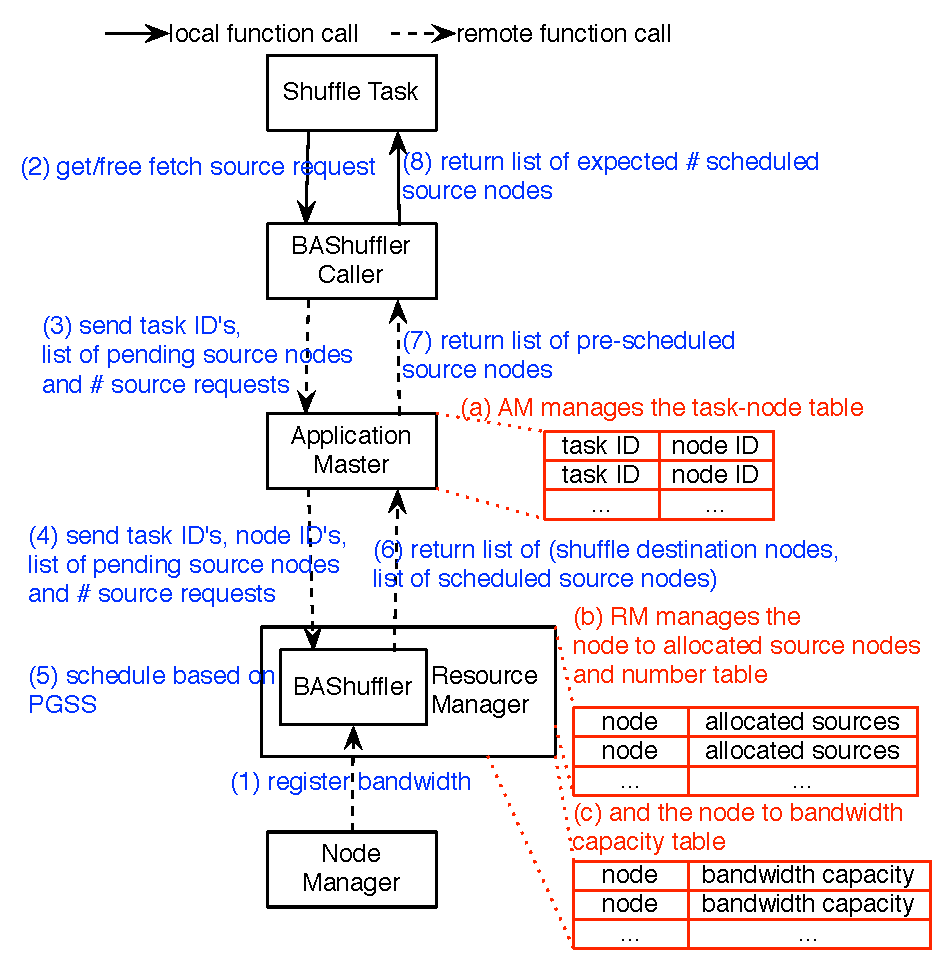
\includegraphics[width=1\columnwidth]{figure1}

\caption{The Architecture of BAShuffler and Shuffle-Related Information Maintained in Components}
\label{fig:bashuffler}
%\vspace{-0.2in}
\end{figure}

At startup, node managers register with BAShuffler the bandwidth capacity of 
the uplinks and downlinks of the nodes (S1). Users can obtain the
capacities of these access layer links of the nodes either from the
specification of the cluster configuration or simply by a bandwidth
evaluation tool.

When a shuffle task needs to schedule a new fetch, with the node executing the shuffle task as the destination node, it initiates a request to the application master
for a scheduled fetch (S2).
The request contains the shuffle information, including 
the shuffle task ID, the list of pending source nodes for fetching
data and the amount of source nodes to request.
% the remote BAShuffler
% to decide the source node to schedule, from a set of available nodes that has finished some map task.
% The BAShuffler caller sends the necessary shuffle information to the
% corresponding application master,
% including the shuffle task ID, the list of pending nodes to fetch
% the data from and the request number of source nodes.
When the application master receives the shuffle scheduling request, 
it caches the request and extracts the node information from the job
information maintained in the application master.
In a heartbeat from the application master to the resource manager,
besides the original container allocation requests
of YARN, the application master also sends those shuffle source
scheduling requests to BAShuffler (S3).
BAShuffler applies a shuffle scheduling policy (PGSS or GSS) to select sources of shuffle tasks, which will be introduced soon. 
% BAShuffler is a centralized scheduler and makes the source scheduling decision based on 
% bandwidth capacities of links and the scheduling status of the whole cluster, e.g., the records of the source and
% destination nodes of the scheduled flows, 
% with the fact that this information is easily at hand of the resource manager.
When the source nodes are selected, BAShuffler will
update the current scheduling status and
the result is transferred back to the shuffle task in the reversed path (S4 and S5). 

When the shuffle task finishes fetching the data from a source and
wants to free the flow,
it will ask BAShuffler to update the source scheduling
status in BAShuffler along the same path.

When a node manager is added to or deleted from the cluster, 
the node manager registers or deregisters its link capacity information 
(and also the existing flow information when deregistering) with BAShuffler, 
just as at startup. 
Adding or deleting a node in the cluster will not add additional workloads 
for users installing and configuring the system. 


\begin{figure}[!t]
\removelatexerror
\begin{algorithm}[H]
\SetKwInOut{Input}{Input}
\SetKwInOut{Output}{Output}

 \Input{$Sources$: source nodes to select; \\
 $Pattern$: sources and destinations of the allocated flows in the cluster;}
 \Output{$Selected$;}

 \If{GSS}{
 	$Nodes$ $\gets$ $Sources$
 } \ElseIf{PGSS}{
 	$Nodes$ $\gets$ the heaviest-loaded source nodes in $Sources$;
 }
 % $Heaviest$ $\gets$ the heaviest-loaded source nodes in $Sources$;\\
 $MaxBandwidth$ $\gets$ 0;
 
 \ForEach{$Source$ $\in$ $Nodes$}{
  $Util$ $\gets$ the MMF bandwidth utilization of the whole cluster after adding $Source$ to $Pattern$;
  
  \If{Util $>$ MaxBandwidth}{
    $MaxBandwidth \gets Util$;\\
    $Selected \gets Source$;
  }
 }
\If{PGSS}{
	update the load count of $Selected$;
}
add $Selected$ to $Pattern$;
\caption{Greedy Source Selection and Partially Greedy Source Selection}
\label{algo:PGSS}
\end{algorithm}
%\caption{Pseudo Code of the Partially Greedy Source Selection Algorithm}
\end{figure}



\subsection{Greedy Source Selection}
A straightforward method to improve the shuffle throughput when
selecting the source is
to use the greedy method for online scheduling: 
whenever there is a new fetch to schedule, the shuffle selects the
pending source node such that after selecting it,
the MMF bandwidth of the whole cluster is no less
than that
when any other pending source node is selected. We call this shuffle
scheduling policy Greedy Source Selection, or GSS. 
Algorithm~\ref{algo:PGSS} presents the procedure of GSS.
%as against the RSS policy of YARN. 

GSS selects the source node that currently maximizes the cluster MMF bandwidth.
GSS is an effective method when it is not the
worst case:
the selections of shuffles concentrate on a part of the pool of the
nodes too much
so that later on, the selection of the remaining source nodes of all
the shuffles can only be concentrated in the other part of the pool.
In this case, in the latter period of source scheduling,
the bandwidth of some nodes cannot be used at all as all the map
outputs have already been fetched.
The total bandwidth utilization might fall dramatically in this worst case. 

\subsection{Partially Greedy Source Selection}
Just like other online scheduling algorithms~\cite{wu2007scheduling, sgall1998line}, 
GSS does not predict the arrival pattern of coming source nodes. 
It makes sure that the maximum transfer throughput of the whole
cluster is achieved at the moment it makes the scheduling decision,
% during the short period
% following the selection of each source,
but it cannot guarantee the maximum average throughput of the cluster
over a long period of time.

A better shuffle source scheduling algorithm is possible if it can
predict the arrival pattern of the source nodes in the future. %to fetch.
There is, however, almost no way to know the arrival pattern of the shuffle
tasks in advance
as when and where a shuffle task starts depends on the allocation of
the reduce container, which is a stochastic process.
Nevertheless, after a shuffle has started, the future pairs of the
sources and the destination of fetch flows can be approximately predicted.
The destination of these fetch flows is the node where the shuffle task
executes,
and the sources are the nodes %where there are input data for the
where 
the map tasks of the same job execute 
(we ignore the case when there happens to be no map output partition
for the shuffle, which is almost impossible
for reasonably large input datasets). 

Therefore, we adjust GSS with future prediction to what we call Partially
Greedy Source Selection (PGSS), whose algorithm is also shown in Algorithm~\ref{algo:PGSS}.
PGSS marks each node with a \emph{load count}, which indicates how many fetch flows will be created by
this source nodes in the near future.
When a shuffle begins, PGSS predicts that there will be a new fetch
flow later from every map task.
Therefore, it increments the load count of each future pending
source node by the number of map tasks of in that source node.
The source nodes with the highest load count is labeled as the heaviest-loaded nodes.
When PGSS needs to select a source from the pending nodes, 
it zeros in on the set of heaviest-loaded nodes first (``partial'') and selects the one that gives that maximum MMF
bandwidth utilization (``greedy'').

\subsection{Comparing GSS and PGSS}
PGSS may not deliver larger overall bandwidth utilization as compared to GSS, 
as PGSS only selects source nodes from the heaviest-loaded
sources, which are in a subset of the domain of GSS.
When the pending source list is long, GSS may concentrates its selection on 
a set of sources that are not heavy-loaded first, in order for the maximum MMF allocation. 
But later in the long run, the remaining sources are heavy-loaded and the throughput of GSS
slows down and the shuffle progress starts to drag. 
PGSS better resolves the dragging case. 


%However, PGSS can better avoid the concentration of selection from a small set
%of sources,
%while maintaining the competitive bandwidth utilization, especially in the long run. 
%Another advantage of PGSS against GSS is that PGSS may incur
%even a smaller scheduling overhead, 
%as PGSS only selects the source nodes from the heaviest-loaded nodes. 

\ref{section:virtualTestbed}

\begin{table}[!t]
% increase table row spacing, adjust to taste
\renewcommand{\arraystretch}{1}
\setlength\tabcolsep{1.5pt}
% \extrarowheight as needed to properly center the text within the cells
\caption{Time Complexity of Different Scheduling Algorithms for Scheduling Each Request}
\label{table:complexity}
\centering
% Some packages, such as MDW tools, offer better commands for making tables
% than the plain LaTeX2e tabular which is used here.
%\begin{tabular}{|c||c|c|}
\begin{tabularx}{.47\textwidth}{c|c|c|c}
\hline
\textbf{RSS} & \textbf{GSS} & \textbf{PGSS} &\textbf{Online Optimal}\\
\hline
$O(1)$ & $O(M \cdot (N+F))$ &
$O(K \cdot (N+F))$ &$O(\frac{(P+M-1)!}{P \cdot P! \cdot(M-1)!} \cdot (N+F))$\\
\hline
\end{tabularx}
%\end{tabular}
\end{table}

Although GSS and PGSS are not the online optimal scheduling solutions for the
shuffle source selection problem,
they are much simpler in terms of time complexity than the online
optimal solution. 
Suppose that the number of nodes in the cluster is $N$,
and during the shuffle, at a specific scheduling moment, 
the number of existing flows in the network is $F$.
$P$ fetchers are
requesting from the set of pending sources of size $M$ at the same time.
The number of the heaviest-loaded nodes is $K(K \leq M)$.
The online optimal solution considers every $P$-combination with $M$ repeated source nodes and then choose the combination that obtains the maximum MMF bandwidth utilization.  
Given that the time complexity for obtaining the MMF
bandwidth utilization
of a specific network from a communication pattern is $O(N+F)$, 
the time complexities of different shuffle source scheduling algorithms for scheduling a fetcher are summarized in Table~\ref{table:complexity}.
RSS, by random selection, gives the least time complexity. 
The time complexities of GSS and PGSS are much smaller than that of the online optimal algorithm.
Generally, PGSS suffers even less scheduling overhead than GSS. 
It is verified in Section~\ref{section:evaluation} that the PGSS
gains performance close to the online optimal but with a much smaller scheduling overhead.

The choice between GSS and PGSS will be discussed in Section~\ref{section:virtualTestbed} accompanied with experiment results. 
In short, PGSS is the better choice for heavily communication-intensive scenarios (traffic predictable) and large-scale clusters (lower overhead). 
While GSS is more suitable for higher bandwidth networks (so that pending source list is short) and smaller-scale clusters.

Currently, GSS and PGSS do not differentiate the fetch flows belonging to different shuffle tasks or different jobs during scheduling. 
It schedules each fetch to maximize the MMF utilization for the whole cluster, but not just for the job that the fetch belongs to. 
Also, GSS and PGSS do not consider the workload size of the flows (the data size to transfer in the flow), as the bandwidth utilization efficiency instead of the flow completion time is the major concern of BAShuffler. 
In fact, the shuffle fetch flows are not batched tasks as some fetch flows are unknown yet and the future flow tasks can come dynamically at casual time.
It is unpractical to consider the shuffle completion time as the performance goal for the online flow tasks.
The goal of maximizing bandwidth utilization is reasonable in the shared environment, e.g., in multi-tenant clusters, and we believe that higher overall bandwidth utilization will lead to shorter completion time.



\begin{figure}[!t]
\centering

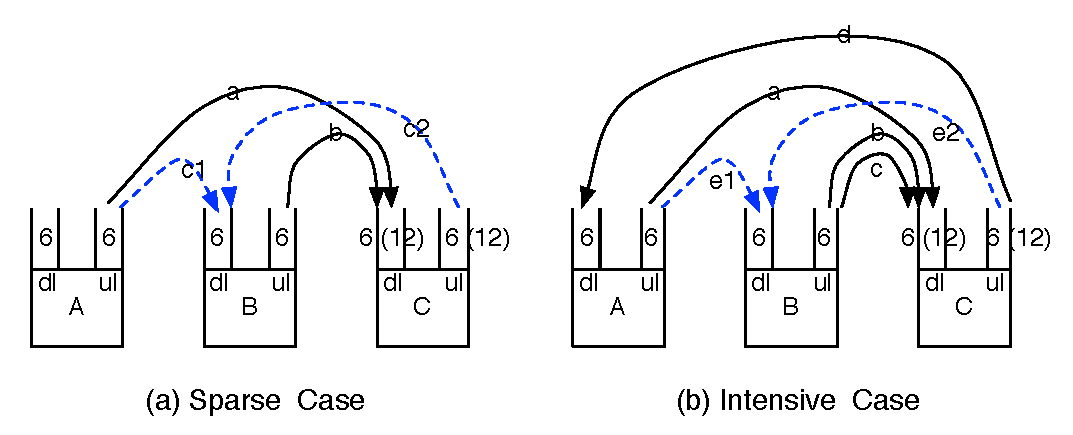
\includegraphics[width=1\columnwidth]{figure3}

\caption{Scenarios of Selecting the Source in Uneven Flow Pattern}
\label{fig:network}
%\vspace{-0.2in}
\end{figure}

\subsection{Applying GSS/PGSS}\label{section:analysis}
We illustrate how GSS or PGSS are applied when selecting a source based on the
MMF allocation in both homogeneous and heterogeneous
network settings, which are distinguished by whether the capacities
of the access layer links are the same or not, respectively.
The analysis can easily extend to a large scale of nodes and flows in
the datacenter, as the MMF behavior follows the same
method of estimation.
%As dicussed in Section~\ref{section:MMF}, 
We assume that the bottleneck links of the TCP
flows are the access links to computer nodes.
Since GSS and PGSS are similar except that PGSS selects source nodes from the heaviest-loaded nodes,
we illustrate the benefit of MMF of estimation in BAShuffler by assuming all nodes are already heaviest-load nodes. 
GSS behaves exactly the same as PGSS then, and for simplicity, we only discuss about applying PGSS.
% We consider both the homogeneous and the heterogeneous network settings,
% which are distinguished by whether the capacities
% of the access layer links are the same or vary.
%i.e., a homogeneous network environment. 
% Although RSS can distribute the
% flows more or less evenly, %to some extent,
% it cannot guarantee exactly the same workload (or number of flows) on each node. 



Fig.~\ref{fig:network} depicts 
two scenarios of the uneven flow pattern, where uneven means
that the numbers of flows into or out of the nodes are different, and even otherwise. 
In the sparse case, some links are idle, while in the intensive case, the
links are almost saturated by the flows.
In the homogeneous network setting,
the three nodes, A, B, and C, have the same uplink and downlink bandwidth
capacities, % which are listed in Table \ref{table:networkSetting}.
which are all 6; whereas in the heterogeneous setting,
their capacities are 6, 6 and 12, respectively.
The solid arrows represent the existing fetch flows and the dashed arrows represent the newly coming flows that can be selected. 
Now, a fetcher in Node B becomes available and PGSS needs to decide a source
node (A or C) to fetch data. 
Assume that both Node A and Node C are the heaviest-loaded nodes.



\begin{table}[!t]
% increase table row spacing, adjust to taste
\renewcommand{\arraystretch}{1}
% \extrarowheight as needed to properly center the text within the cells
\caption{MMF Flow Allocation of the Sparse Case in Homogeneous Network}
\label{table:homoSparse}
\centering
% Some packages, such as MDW tools, offer better commands for making tables
% than the plain LaTeX2e tabular which is used here.
%\begin{tabular}{|c||c|c|}
\begin{tabularx}{.35\textwidth}{c||c|c|c|c|c}
\hline
\textbf{Selected Flow} & \textbf{a} & \textbf{b} & \textbf{c1} & \textbf{c2} & \textbf{Overall}\\
\hline
Nil &3&3&-&-&6\\
\hline
c1 &3&3&3&-&9\\
\hline
c2 &3&3&-&6&12\\
\hline
\end{tabularx}
%\end{tabular}
\end{table}

\begin{table}[!t]
% increase table row spacing, adjust to taste
\renewcommand{\arraystretch}{1}
% \extrarowheight as needed to properly center the text within the cells
\caption{MMF Flow Allocation of the Intensive Case in Homogeneous Network}
\label{table:homoIntensive}
\centering
% Some packages, such as MDW tools, offer better commands for making tables
% than the plain LaTeX2e tabular which is used here.
%\begin{tabular}{|c||c|c|}
\begin{tabularx}{.42\textwidth}{c||c|c|c|c|c|c|c}
\hline
\textbf{Selected Flow} & \textbf{a} & \textbf{b} & \textbf{c} & \textbf{d} & \textbf{e1} &\textbf{e2} &\textbf{Overall}\\
\hline
Nil &2&2&2&6&-&-&12\\
\hline
e1 &2&2&2&6&4&-&16\\
\hline
e2 &2&2&2&3&-&3&12\\
\hline
\end{tabularx}
%\end{tabular}
\end{table}


\subsubsection{Homogeneous Network}
Different selection decisions lead to different flow bandwidth allocations and overall bandwidth utilizations. 
In the homogeneous network setting, the MMF bandwidth
allocation of each flow before or after selecting a new flow is
shown in Table \ref{table:homoSparse} (for the sparse case) and Table
\ref{table:homoIntensive} (for the intensive case), respectively, where ``Nil'' in an entry means the status before the source selection.
In the sparse case (Fig.~\ref{fig:network}), PGSS selects Node C as the source, which offers 33\% higher overall
bandwidth utilization than if Node A is selected.
Note that the RSS policy of YARN will have a 50\% probability of selecting
Node A, not guaranteeing the maximum utilization of the bandwidth
even in the homogeneous network setting.
%Usually, there are lots of such idle bandwidth that can be made use of
%if the shuffle carefully selects the source node for fetching data. 

Applying MMF to estimate the bandwidth allocation can
help make better decisions when selecting the source nodes at the
application level.
In the intensive case (Fig.~\ref{fig:network}), if we assume that the upload (download)
rates of flows are only decided by the uplink (downlink)
capacity and the number of the flows sharing that link
as in \cite{chowdhury2011managing},
it will make no difference whether to choose Flow e1 or Flow e2,
as both source nodes have one outgoing flow from them 
(Flow a and Flow d). 
However, by the notion of MMF, PGSS will select e1 that can maximize the overall bandwidth utilization. 



\begin{table}[!t]
% increase table row spacing, adjust to taste
\renewcommand{\arraystretch}{1}
% \extrarowheight as needed to properly center the text within the cells
\caption{MMF Flow Allocation of Uneven Pattern in Heterogeneous Network}
\label{table:heteUneven}
\centering
% Some packages, such as MDW tools, offer better commands for making tables
% than the plain LaTeX2e tabular which is used here.
%\begin{tabular}{|c||c|c|}
\begin{tabularx}{.35\textwidth}{c||c|c|c|c|c}
\hline
\textbf{Selected Flow} & \textbf{a} & \textbf{b} & \textbf{c1} & \textbf{c2} & \textbf{Overall}\\
\hline
Nil &6&6&-&-&12\\
\hline
c1 &3&6&3&-&12\\
\hline
c2 &6&6&-&6&18\\
\hline
\end{tabularx}
%\end{tabular}
\end{table}

\subsubsection{Heterogeneous Network}
In the heterogeneous network setting, the randomly source selection policy
can even have an greater (negative) impact on the
bandwidth utilization than in a homogeneous network, 
no matter whether the flows are evenly allocated across the network or not.

%\subsubsection{Uneven Flow Pattern}
Look at the uneven flow patterns in Fig.~\ref{fig:network} again. 
In the heterogeneous network setting, 
the MMF bandwidth allocation of each flow is shown in Table~\ref{table:heteUneven}.
The overall bandwidth utilization difference between selecting Flow c1 and Flow c2 is amplified in the heterogeneous network (3:2),
as compared to the homogeneous network (4:3).
PGSS will always select the source (Node C) that brings about the maximum
bandwidth utilization.

In the homogeneous network, if the communication pattern of the flows
is exactly even, that is
where every link has the same number of flows, selecting any source
node for fetching
will make almost no difference in the overall bandwidth utilization. 
However, in the heterogeneous network, selecting the right source node
is critical for high bandwidth utilization.

\begin{figure}[!t]
\centering

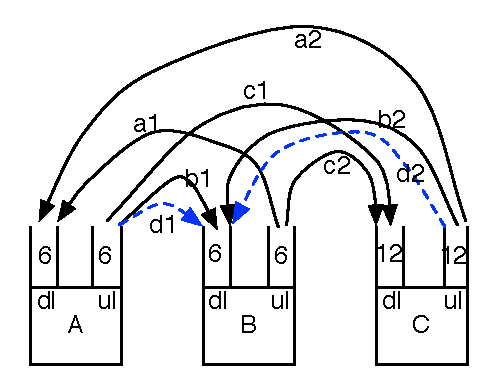
\includegraphics[height=0.35\columnwidth]{figure4}

\caption{Selecting the Source in the Even Flow Pattern}
\label{fig:network3}
%\vspace{-0.2in}
\end{figure}
 
Fig.~\ref{fig:network3} depicts the scenario of the even flow pattern, and the capacities of the links follow the heterogeneous setting.
%We analyze the bandwidth utilization in the even flow pattern
%scenario as shown in Fig.~\ref{fig:network3}. 
The MMF allocation of the flows before and after
selecting the new dashed flows is shown in Table
\ref{table:heteEven}.
Surprisingly, it does happen that the overall MMF bandwidth utilization
drops if Flow d1 is selected.
PGSS selects Flow d2 to guarantee the maximum bandwidth utilization.

\begin{table}[!t]
% increase table row spacing, adjust to taste
\renewcommand{\arraystretch}{1}
% \extrarowheight as needed to properly center the text within the cells
\caption{Max-Min Fairness Bandwidth Allocation of Flows of Even Flow Pattern in Heterogeneous Network Setting}
\label{table:heteEven}
\centering
% Some packages, such as MDW tools, offer better commands for making tables
% than the plain LaTeX2e tabular which is used here.
%\begin{tabular}{|c||c|c|}
\begin{tabularx}{.45\textwidth}{c||c|c|c|c|c|c|c|c|c}
\hline
\textbf{} & \textbf{a1} & \textbf{a2} & \textbf{b1} & \textbf{b2} & \textbf{c1} &\textbf{c2}& \textbf{d1}& \textbf{d2} &\textbf{Overall}\\
\hline
Nil &3&3&3&3&3&3&-&-&18\\
\hline
d1 &3&3&2&2&2&3&2&-&17\\
\hline
d2 &3&3&2&2&4&3&-&2&19\\
\hline
\end{tabularx}
%\end{tabular}
\end{table}

Overall, neither RSS nor selecting the source based on the number of flows on
the link makes the right decision that
maximizes the bandwidth utilization in the MMF network.
However, by applying the knowledge
of the bandwidth capacities of the
access layer links and the TCP flow communication patterns (sources
and destinations of the flows),
PGSS can easily find out the proper source node to achieve the maximum
transfer throughput of the flows by
the behavior of MMF.


\subsection{Implementation Details}

\textbf{Rearranging Selecting Sequence}: PGSS applies the ``first-hit" approach when selecting the source node. 
For a specific sequence of the pending source nodes, PGSS will always
prefer the source node in the front of the sequence
among the source nodes with the same maximum bandwidth utilization
if they are selected.
%after selected.
To avoid the case that the source nodes in the front
of the sequence starves the nodes in the tail,
PGSS rearranges the sequence of the pending source nodes randomly
before it starts to find the first-hit node.
This guarantees that every source node that can achieve the maximum
bandwidth has the same chance to be selected.
% , and
% reduces the probability of concentration during the latter period of
% scheduling.

\textbf{Pre-Scheduling}:
Usually, the shuffle task has only one free fetcher at a time,
and the shuffle requests for a scheduled source from BAShuffler every time (Fig.~\ref{fig:bashuffler}). 
For every source request from the shuffle task to BAShuffler, 
it takes two segments of remote call time, one segment of heartbeat
interval time and two segments of thread scheduling time.
In fact, the pending sources for fetching are known before free
fetchers ask for the sources.
BAShuffler uses the \emph{pre-scheduling} strategy, which requests
a number of the scheduled sources from BAShuffler at a time,
and when a fetcher needs a source, the shuffle task can return one
immediately. Although the actual flow pattern may lag slightly behind
the scheduling pattern stored in BAShuffler when pre-scheduling,
the pattern will quickly catch up when the scheduled sources in the cache of
the shuffle task are consumed.


\section{Evaluation}\label{section:evaluation}
To evaluate the performance of BAShuffler, 
we conduct experiments in a physical cluster of heterogeneous
network setting with realistic benchmarks and datasets.
The performance improvement of BAShuffler will also be verified in an
Amazon EC2 virtual cluster, whose underlying network setting is
unknown to users.
Furthermore, we also evaluate the scalability of BAShuffler in
clusters of different scales and degrees of heterogeneity by simulation.


\begin{table}[!t]
% increase table row spacing, adjust to taste
\renewcommand{\arraystretch}{1}
% \extrarowheight as needed to properly center the text within the cells
\caption{Benchmark Dataset Size (GB)}
\label{table:benchmark}
\centering
% Some packages, such as MDW tools, offer better commands for making tables
% than the plain LaTeX2e tabular which is used here.
%\begin{tabular}{|c||c|c|}
\begin{tabularx}{.4\textwidth}{c||c|c|c}
\hline
\textbf{Benchmark} & \textbf{Input} & \textbf{Shuffle} & \textbf{Output} \\
\hline
Terasort & 190 & 190 & 190\\
\hline
InvertedIndex & 200 & 42 & 34 \\
\hline
%SequenceCount & 200 & 190 & 150 \\
SequenceCount & 300 & 180 & 150 \\
\hline
RankedInvertedIndex & 150 & 175 & 153\\
\hline
\end{tabularx}
%\end{tabular}
\end{table}

\subsection{Physical Testbed}
% To verify the benefits of BAShuffler in scheduling the shuffle fetch
% flows with awareness of the network bandwidth allocation behavior,
%we run BAShuffler in real testbeds, including a physical cluster and
%a virtual cluster with heterogeneous networks.
We run BAShuffler in a physical testbed, the
Gideon-II cluster \cite{gideon} in the heterogeneous network configuration.
The physical testbed is a cluster containing 18 computer nodes, where one node
assumes the role of the name node of HDFS, and
one node acts as the resource manager of YARN. 
The remaining 16 nodes are configured as both the data nodes of HDFS
and the node managers of YARN.
Each node is equipped with 2 quad-core, 32 GB DDR3 memory and
2 $\times$ 300 GB SAS hard disks running RAID-1. 
All the 18 nodes run with Scientific Linux 5.3 and are connected to an internal non-blocking switch with GbE ports. 
To create the heterogeneous network capacity, among 16 node managers, 
the bandwidth capacity of the uplinks and downlinks of 8 nodes is
manually limited to 160 Mbps,
by using the traffic control tool ``\emph{tc}'', 
and the remaining 8 nodes keep to their physical uplinks and downlinks
bandwidth capacity, which is 320 Mbps.


\begin{figure}
\centering
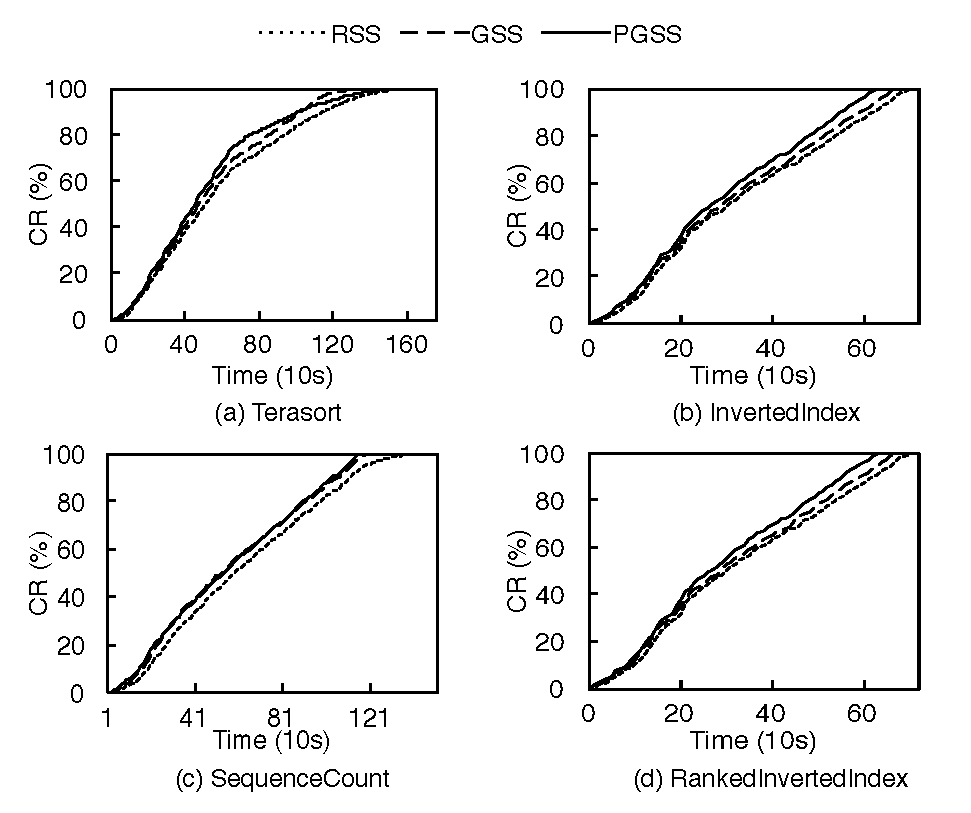
\includegraphics[width=1\columnwidth]{figure5}
\caption{Cumulative Completion Ratio (CR) of the Overall Shuffle Workload of RSS, GSS and PGSS in Various Benchmarks along the Time
in the Physical Testbed} 
\label{fig:new_completion_ratio}
\end{figure}


The benchmarks and datasets used are from a realistic MapReduce benchmark suite~\cite{ahmad2012puma}. 
We use mainly the shuffle-heavy applications because we want to evaluate  BAShuffler when the shuffle workload can saturate the
network most of the time. 
BAShuffler performs almost the same in shuffle-light applications in the benchmark suite and we leave them out in the experiment results. 
% and ignore the other applications whose shuffle workloads are quite
% low. %regarding the input data size.
The sizes of the datasets of the benchmarks are listed in Table \ref{table:benchmark}.

BAShuffler is configured in advance to know
the link bandwidth capacity of each node.
%We run the typical shuffle-heavy MapReduce job, i.e., SequenceCount \cite{ahmad2012puma} on YARN, 
%with both the original shuffle scheduler and BAShuffler. 
Unless specified otherwise, %the input data size for each job is 200 GB, 
in both the physical testbed and the virtual testbed introduced later, 
the number of fetchers in each shuffle task is 5 (the default value), 
the number of reduce tasks of each job is configured to
be the total number of node managers in the cluster, 
and other Hadoop configurations keep their default values. 
We compare GSS and PGSS with RSS, and RSS is the default and the only
presently known application-level shuffle scheduler in YARN. 
The following sub-sections report the overall shuffle throughput of
the cluster, the shuffle rate of each shuffle task, the reduce phase
completion time and the job overall completion time.
We also measure the performance of BAShuffler with input data of
different sizes
and the performance in the shared environment with multiple concurrent jobs. 
The results will be introduced later together with the those of the virtual cluster. 

\begin{figure}
\centering
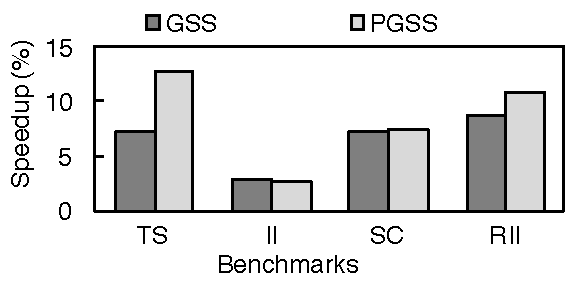
\includegraphics[width=0.7\columnwidth,height=0.35\columnwidth]{figure6}
\caption{GSS and PGSS Speedup of Average Shuffle Rate of Each Shuffle Task in comparison to RSS in Benchmarks Terasort (TS), InvertedIndex(II), SequenceCount (SC) and RankedInvertedIndex (RII) in the Physical Testbed} 
\label{fig:new_shuffle_rate}
\end{figure}

\subsubsection{Shuffle Throughput}
The throughput performance of GSS and PGSS can be measured by the overall shuffle
throughput of the cluster
and the average shuffle rate of each shuffle task, respectively. 
We use the metric of the overall shuffle throughput because it
reflects the cluster overall bandwidth utilization along the time axis.
The start time and finish time of the shuffle tasks are usually different from each other during the shuffle phase, but can also overlap. 
The average shuffle rate of each shuffle task, on the other hand, reflects how each individual shuffle task can benefit from the throughput increase of the cluster.

The overall shuffle throughput is depicted as the cumulative
completion ratio of the overall shuffle workload.
Fig.~\ref{fig:new_completion_ratio} shows the results of RSS, GSS
and PGSS in various benchmarks in the physical cluster.
GSS and PGSS outperform RSS in all benchmarks, 
and PGSS even performs better than GSS in most cases. 
In the SequenceCount benchmark, GSS and PGSS have similar shuffle
throughputs, %along the time,
which shows that the simple greedy method can also maximize the
bandwidth utilization in some cases,
as long as that it selects the fetch source node based on the estimation of the bandwidth allocation status. 
The overall shuffle throughput improvement is the result of improved overall bandwidth utilization.

One thing to notice is that we can see slightly longer tails in the shuffle CR line (e.g., RSS and GSS in Terasort and RSS in SequenceCount). 
It is because a few of the shuffle tasks unfortunately gain lower throughput at the beginning. When some other tasks finish shuffling, they still cannot increase the throughput and become stragglers. The reason is that the largest throughput these remaining stragglers can attain depends on the bandwidth of the working links, but not the bandwidth of the whole cluster. As a result, the transfer rate is slow and we see the tails.

The comparison of the average shuffle rates of shuffle tasks between GSS, PGSS and RSS is made based on the speedup factor. 
The speedup is calculated by the average shuffle rate difference between GSS (or PGSS) and RSS over that of RSS. 
The results are shown in Fig.~\ref{fig:new_shuffle_rate}.
GSS and PGSS gain relatively high shuffle rate speedups as compared to
RSS in all benchmarks, which are about 7\% and 12\% in the
Terasort benchmark.
The speedups of PGSS are a bit higher than GSS, e.g., in Terasort (by 5\%) and RankedInvertedIndex (by 3\%). 



\subsubsection{Completion Time}
We also measure how much the job completion time can be decreased by maximizing the network bandwidth utilization with GSS and PGSS. 
The reduce completion time is the time period between the time when all the
map tasks have finished and the time the job finishes.
During the reduce completion time, no map task is running, and most of
the tasks are doing the shuffle work at the first half of the time and
doing the reduce work at the second half of the time.
We did not observe the metrics of ``shuffle completion time'' because
the tasks finish the shuffle work at different times and it is hard to
define the endpoint of the shuffle completion time.


\begin{figure}
\centering
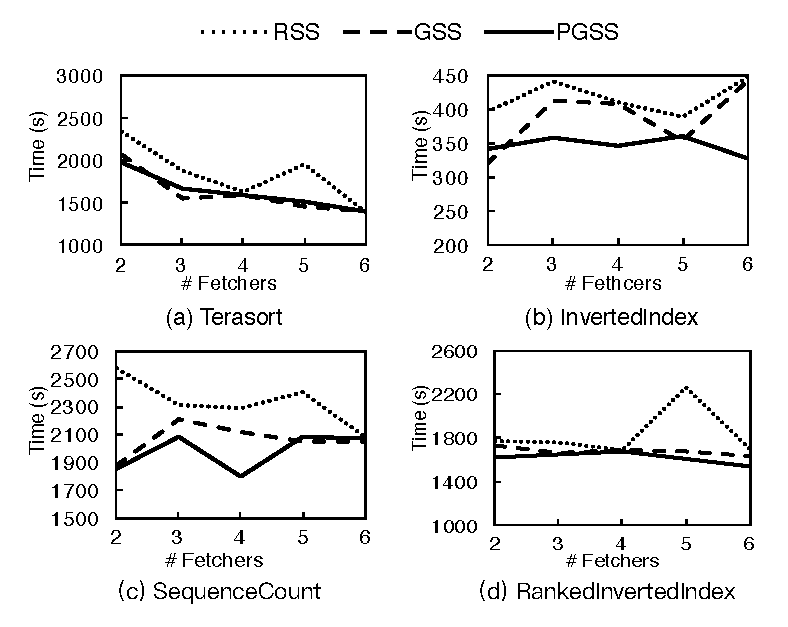
\includegraphics[width=1\columnwidth]{figure7}
\caption{Reduce Completion Time of RSS, GSS and PGSS in Various Benchmarks with Different Numbers of Fetchers in Each Shuffle Task
in the Physical Testbed} 
\label{fig:new_reduce_completion}
\end{figure}


\textbf{Reduce Completion Time:} The reduce completion time of RSS, GSS and PGSS in various benchmarks with different numbers of fetchers in shuffle tasks are shown in Fig.~\ref{fig:new_reduce_completion}. 
Different numbers of fetchers will create different degrees of traffic
congestion in the network. 
The case of only one fetch in each shuffle task is skipped because the
sparse communication pattern will leave some of the links idle.
The results show that PGSS takes significantly less
time to complete the reduce than RSS.
The exact speedup is depicted in Fig.~\ref{fig:new_speedup} and will be described soon.
The reduce completion time of RSS with different numbers of fetchers
deviates from each other over a large value range without obeying following an obvious pattern,
which indicates that RSS is sensitive to different levels of network traffic
congestions.
The reduce completion time of GSS and PGSS is more flat
with different numbers of fetchers in all benchmarks.
Except in Terasort, where PGSS and GSS are close in reduce completion time,
PGSS generally performs better than GSS with different fetcher numbers in the other benchmarks. 
PGSS is more applicable to various traffic congestion statuses.

It is not our work to obtain such an ``optimal'' fetcher number that generates the least reduce time because it seems unpredictable from the results of different benchmarks or just may not be unique 
(e.g., 4 fetchers and 6 fetchers in RankedInvertedIndex generate almost the same reduce time, and it is hard to tell the fetch number is an important impact factor for the same reduce time), which indicates that the obtaining the ``optimal'' fetcher number may be a false proposition.
Besides, even if there is such an ``optimal'' fetcher number for RSS, it requires users multiple runs to obtain such number, and the best reduce completion time is narrowly shorter than the worst one with PGSS in the Terasort Case. 
While in the other benchmarks, PGSS's worst result is no worse than the best one of RSS with any fetcher number. 



\textbf{Overall Completion Time:} Fig.~\ref{fig:new_speedup} depicts the reduce completion time speedup
and the job overall completion time speedup of GSS and PGSS as
compared to RSS with different numbers of fetchers in each shuffle
task.
The completion time speedup is calculated based on the time difference between GSS (or PGSS) and RSS over the time of RSS. 
As the benchmarks are reduce-heavy, where the shuffle phase occupies
a major portion of the overall workload, in most cases, BAShuffler not
only improves the reduce phase, but also the overall
completion time of the jobs by a remarkable margin.
For example, in the RankedInvertedIndex benchmark with 5 fetchers, 
GSS and PGSS decrease the reduce completion time by 26\% and 29\%, respectively, 
and decrease the overall completion time by 19\% and 21\%, respectively.  
We also note that in some cases, the speedups of GSS and PGSS are not obvious (e.g.,
Terasort with 6 fetchers and RankedInvertedIndex with 4 fetchers) when
the reduce completion time of RSS is already the minimum among all the
fetcher settings.


\begin{figure}[!t]
\centering
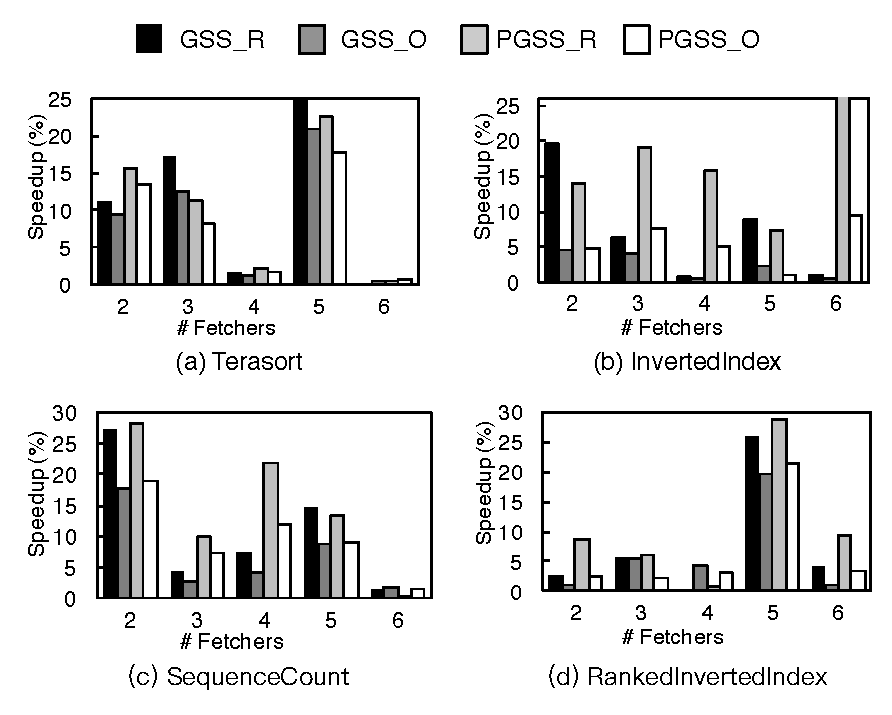
\includegraphics[width=1\columnwidth]{figure8}
\caption{Reduce Completion Time Speedup (Suffixed with \_R) and Job Overall Completion time Speedup (Suffixed with \_O) of GSS and PGSS as Compared to RSS in Various Benchmarks with Different Fetcher Numbers
in the Physical Clusters}
\label{fig:new_speedup}
%\vspace{-0.22in}
\end{figure}

\subsection{Virtual Testbed}\label{section:virtualTestbed}
The virtual testbed is meant to evaluate the performance of BAShuffler in the environment when the network settings are unclear. 

We deploy the virtual testbed on Amazon EC2, with a cluster consisting of 9 c3.xlarge
instances and 10 c3.2xlarge instances running
Amazon Linux Image \cite{aws}. The c3.xlarge instance is referred to as the \emph{medium} instance 
and the c3.2xlarge instance the \emph{large} instance below. 
The network topology and configuration of EC2 clusters are unclear, 
but the transfer rates of the access layer links are more or less stable. 
By our measure, the actual uplink and downlink bandwidth capacities of
the medium instance are both about 720Mbps, 
and those of the large instance are about 1000 Mbps. 
One large instance is set up as both the name node of HDFS and the
resource manager of YARN,
and each of the remaining 18 instances, whether medium or large,
is set up as both a data node of HDFS and a node manager of YARN. 

As the performance of BAShuffler in various benchmarks has been
evaluated in the physical cluster
and BAShuffler has similar performance in these benchmarks, in the virtual cluster, 
we use only one benchmark (i.e., SequenceCount, which has the largest
input data size ) for the evaluation for the reason of simplicity and avoiding redundancy.

\subsubsection{Cluster Overall Shuffle Throughput}
Similarly, the overall shuffle throughput of the cluster is described by the cumulative completion ratio of the overall shuffle workload. 
Fig.~\ref{fig:r_vshuffle_timeline} depicts the results of the
SequenceCount benchmark being executed in the virtual cluster, 
where BAShuffler delivers much higher shuffle throughput than RSS. 
A different observation from the physical cluster is witnessed: GSS is faster than PGSS in the virtual case. 
The reason is discussed as follows. 
The network bandwidth capacities of the links in the virtual cluster are much higher than those of in the physical one, with similar CPU rates. 
With the higher shuffle throughput, the length of the list of the pending fetch sources is smaller in the virtual cluster, as the fetch tasks finish faster. 
Although PGSS is designed to prevent the worse
case that some heavy-loaded nodes are starved for a long period, which GSS may encounter, 
GSS is good enough to handle the scheduling of the pending sources of short length. 

It leads us to think of the choice between GSS and PGSS. 
GSS performs well when the pending source list is of short length, which is either because the network throughput is high as compared to the data size that the CPU can generate, or because the shuffle size is relatively low (shuffle-trivial). With the setting that the network would be bottleneck for the job and the workload type is shuffle-heavy, by further considering the lower scheduling overhead in the large-scale cluster (which will be evaluated in Section~\ref{section:eva_overhead}), PGSS is preferred. 


Although the underlying network settings are unclear, the experiment
results show that BAShuffler can also improve the bandwidth
utilization in the EC2 virtual cluster by regarding the virtual
network as a non-blocking switch.

\begin{figure}[!t]
\centering
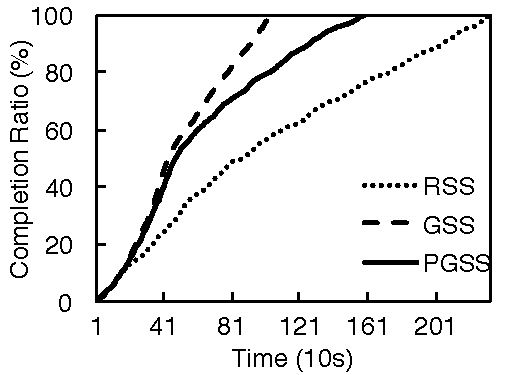
\includegraphics[width=0.7\columnwidth,height=0.4\columnwidth]{figure9}
\caption{Cumulative Completion Ratio of Shuffle Workload in the SequenceCount Benchmark along the Time in the Virtual Cluster}
\label{fig:r_vshuffle_timeline}
%\vspace{-0.22in}
\end{figure}

\subsubsection{Completion Time}
The reduce completion time of the SequenceCount benchmark with different fetcher numbers in the virtual cluster is shown in Fig.~\ref{fig:r_vsequence}. 
Similar to the situation of the physical cluster,
BAShuffler decreases the reduce
completion time in different fetcher number settings.
When the fetcher number is 2, GSS and PGSS decrease the reduce
completion time by 26\% and 8\%, respectively.
The curve of PGSS is more flat than the other scheduling algorithms and is always below that of RSS, which is the same as in the physical cluster.
As discussed in the previous sub-section, GSS generally performs better than PGSS
because of the faster network transfer rate over the CPU rate. 
In the case with 6 fetchers, when the network is more congested, GSS gives merely the same reduce completion time as RSS, but PGSS
decreases the time by about 11\% as compared to RSS. 



\begin{figure}[!t]
\centering
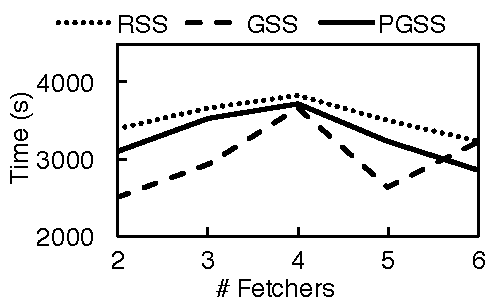
\includegraphics[width=0.7\columnwidth,height=0.4\columnwidth]{figure10}
\caption{Reduce Completion Time of the SequenceCount Benchmark with Different Fetcher Numbers
in the Virtual Testbed}
\label{fig:r_vsequence}
%\vspace{-0.22in}
\end{figure}


\subsubsection{Different Input Data Sizes}
The influence of the application-level shuffle scheduling is contributed by 
the characteristics of the jobs, the varieties in the resource configurations
(e.g., CPU, memory and network) of the cluster, as well as the size of the input data.
To evaluate the scalability of BAShuffler in processing large datasets, 
we run BAShuffler against different sizes of input data for the jobs.
Fig.~\ref{fig:r_sizes} shows the RSS and PGSS reduce completion time of the
SequenceCount Job with different input data sizes
in both the physical and the virtual testbeds. 
Note that the total numbers of nodes of the physical and virtual testbeds are different.
PGSS performs better than RSS in both the testbeds regardless of the input data size. 
The completion time improvement ranges from 8\% to 13\% in the physical testbed
and from 2\% to 17\% in the virtual one. 
 


\begin{figure}[!t]
\centering
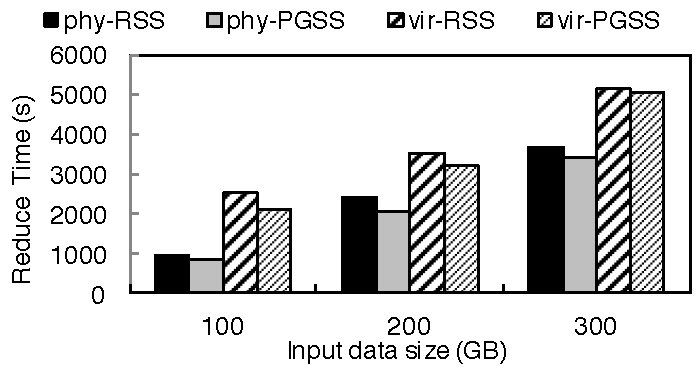
\includegraphics[width=0.8\columnwidth,height=0.4\columnwidth]{figure11}
\caption{Reduce Completion Time of SequenceCount with Different Input Data Sizes in the Physical and Virtual Testbeds}
\label{fig:r_sizes}
\end{figure}



\subsubsection{Multiple Concurrent Jobs}
BAShuffler improves the concurrent job execution time by increasing
the throughput of the concurrent shuffle tasks.
We evaluate how BAShuffler can improve the job completion time when
multiple jobs run concurrently in the shared cluster.
%Finally, we conduct the experiments with multiple concurrent jobs in the cluster. 
We submit three SequenceCount jobs to the clusters at the same time.
%and we submit each job 15 seconds after the previous is submitted. 
The container scheduler is the default Capacity Scheduler in YARN. 
Fig.~\ref{fig:r_concurrent} shows the average job completion time and
the last job completion time of the concurrent jobs.
Note that the times for the physical testbed and the virtual testbed
are in different scales in the figure.
PGSS decreases the average completion time and the last job
completion time by about 6\% and 15\% in the physical testbed 
and by about 7\% and 2\% in the virtual testbed, respectively. 
In the virtual testbed, the second job completion time of PGSS is still 13\% higher than that of RSS, but the final results at ``2\%''.
The reason may be that PGSS has the chance of pending some shuffle tasks of the third job as a penalty of achieving a maximum MMF allocation, 
while RSS is more fair for different jobs but gains poorer average completion time. 


\begin{figure}[!t]
\centering
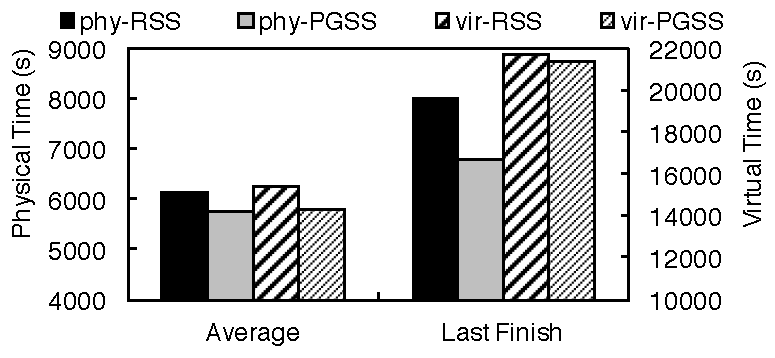
\includegraphics[width=0.9\columnwidth,height=0.4\columnwidth]{figure12}
\caption{Job Completion Time of Multiple Concurrent Jobs in the Physical and Virtual Testbeds}
\label{fig:r_concurrent}
\end{figure}


\subsection{Simulation}
It is hard to measure the performance of BAShuffler in real
testbeds of different scales; we rely on
simulations to provide some insight of algorithmic benefits and
overheads, and the results are convincing.  %with convincing results. 
Different scheduling algorithms generate scheduling decisions
of the source nodes,
and the bandwidth utilization of these scheduling
decisions is calculated based on the MMF mechanism.

We classify the synthetic nodes into low-bandwidth nodes and
high-bandwidth nodes.
The bandwidth capacity of uplinks and downlinks of the
low-bandwidth nodes is 512 Mbps %respectively,
and it is 1024 Mbps for the high-bandwidth ones. Unless specified, 
otherwise, there is one shuffle task running on each node, 
and each shuffle task has 5 fetchers in total. Each shuffle needs to fetch data from all the other nodes in the cluster.
The order of fetch requests is:
one shuffle of the node requests to schedule all its fetch flows,
then another shuffle on another node requests to schedule all its fetches, 
and go on. 
When there is no free fetcher in a shuffle, the shuffle will assume
that a random working fetcher has finished the
fetch, release the corresponding fetch flow, and schedule a new pending
source node for the new free fetcher.
When the shuffle finishes fetching data from all the pending source
nodes, a new shuffle will start on the same node to start to fetch
data from all the other nodes again if it has free fetchers.

All tests about PGSS and the online optimal algorithm are ran
10 times, and it is 100 times for
tests about RSS due to its property of total randomness.
The bandwidth utilization value is obtained as the mean value of all runs.
% There is one shuffle task with 5 fetchers in each node.  
% During the workload, at every time interval, 
% the shuffle on a node will request to schedule the source nodes for
% its free fetchers
% before it is the turn for the shuffle on the next node in the sequence.
Simulation results show that PGSS performs much better than RSS
in bandwidth utilization
with different numbers of nodes and different degrees of network heterogeneity. 


\begin{figure}[!t]
\centering

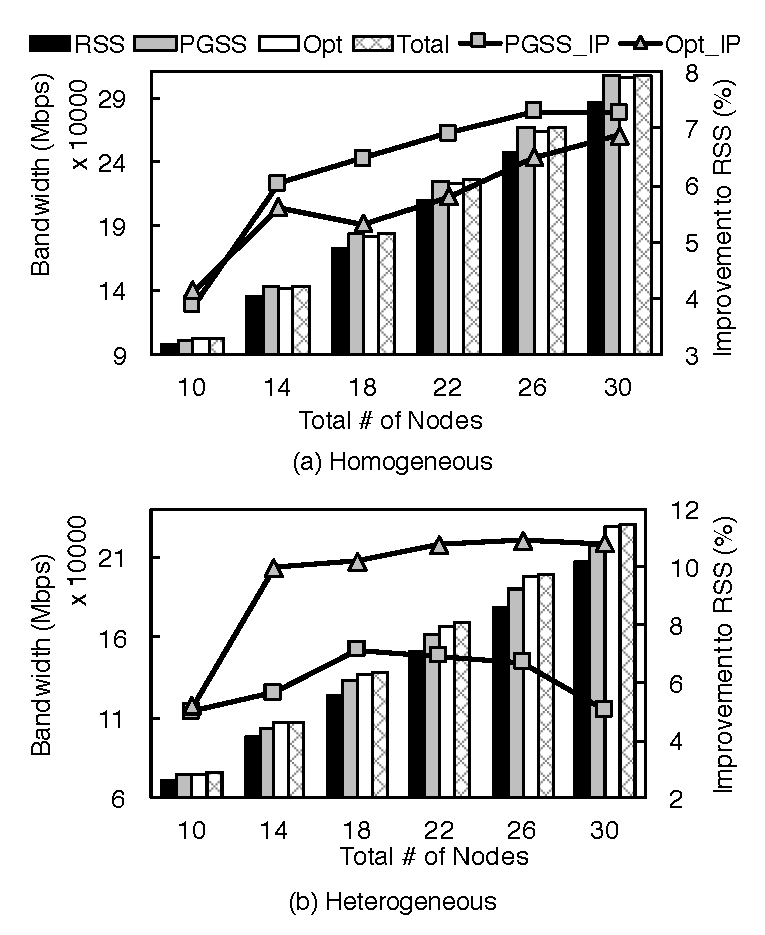
\includegraphics[width=1\columnwidth]{figure13}

\caption{Bandwidth Utilization and Improvement (Suffixed with IP) of RSS, PGSS and the Online Optimal Algorithm (Opt) with Different Amount of Nodes in the Homogeneous Settings and the Heterogeneous Settings}
\label{fig:s_nodes}
\end{figure}

\subsubsection{Different Numbers of Nodes}\label{section:differentNodeNumber}
We first evaluate the performance of PGSS and the online optimal algorithm in clusters of
different scales, i.e., different numbers of nodes.
Both the homogeneous and heterogeneous network modes are tested. 
In the homogeneous mode, all the nodes are high-bandwidth nodes, 
while in the heterogeneous mode, half of them are low-bandwidth nodes
and the other half are high-bandwidth ones.
Fig.~\ref{fig:s_nodes} shows the bandwidth utilization of the homogeneous and
heterogeneous modes,
respectively. 
% The solid line represents the total bandwidth capacities of the links in the cluster in different cases.
The online optimal scheduling solution (Opt) is the maximum online result by traversing every possible permutation of the pending requests that the scheduler have already seen. 
The total bar represents the bandwidth capacities of all the links in the cluster. Two solid curves stand for the improvement of PGSS and Opt as compared to RSS, respectively.
The bandwidth utilizations of both PGSS and Opt 
are about 3.9\% to 7.3\% higher than RSS in the homogeneous mode
and about 5.0\% to 10.9\% in the heterogeneous mode. 
% The improvement in bandwidth utilization of GSS and PGSS is higher 
% in the heterogeneous mode, which is about 5.0\% to 11.0\%. 
% This is because RSS is unaware of the bandwidth allocation status when
% trying to make a scheduling decision. 
An interesting result is that PGSS performs even slightly better than the online optimal algorithm in the homogeneous mode, which is possible as the online optimal algorithm only optimize the bandwidth utilization without considering the pattern of the future fetch flows, while PGSS labels the future fetch flows with the load count. 
In all cases, the bandwidth utilizations of PGSS are close to the total bandwidth capacities.
%In general, the RSS algorithm wastes more proportion of available bandwidths when the total amount of nodes is larger.

\begin{figure}[!t]
\centering

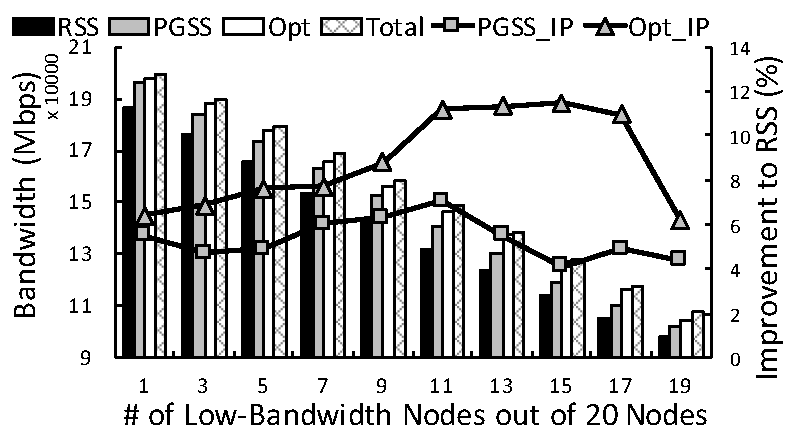
\includegraphics[width=0.8\columnwidth,height=0.4\columnwidth]{figure14}

\caption{Bandwidth Utilization and Improvement (Suffixed with   IP) of RSS, PGSS and the Online Optimal Algorithm (Opt) with Different Degrees of Network Heterogeneity}
\label{fig:s_lowbandwidth}
\end{figure}

\subsubsection{Different Degrees of Network Heterogeneity}
We also evaluate the bandwidth utilization of different source scheduling algorithms 
with different degrees of network heterogeneity, 
i.e., different ratios of low-bandwidth nodes to high-bandwidth ones. 
We run the scheduling algorithms with totally 20 synthetic nodes, 
some of which are low-bandwidth nodes and the rest are high-bandwidth nodes. 
The result is shown in Fig.~\ref{fig:s_lowbandwidth}, 
where the left and the right ends of the horizontal axis stand for a higher
degree in homogeneity
and the middle part of the figure stands for a higher degree in heterogeneity. 
PGSS performs better than RSS in various heterogeneous networks, 
especially with higher degrees in heterogeneity, 
With higher degrees in heterogeneity, the PGSS bandwidth utilization
increase is about 7\% in the simulation. 
It show the benefits of the bandwidth-aware source selecting algorithm in the heterogeneous networks.

\begin{figure}[!t]
\centering

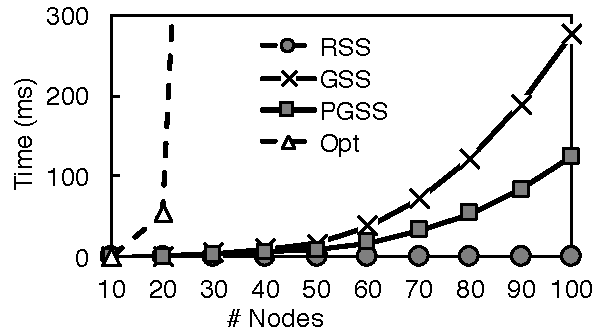
\includegraphics[width=0.7\columnwidth,height=0.4\columnwidth]{figure15}

\caption{Scheduling Overhead Time per Flow of the RSS, GSS, PGSS and Online Optimal (Opt) Algorithms with Different Number of Nodes in the Cluster}
\label{fig:s_overhead}
%\vspace{-0.2in}
\end{figure}

\subsubsection{Scheduling Overhead}\label{section:eva_overhead}
The scheduling overhead of BAShuffler is the time to figure out the source scheduling decision, is related to the number of total nodes and existing flows (whose number generally grows as the number of nodes grows) in the cluster. 
Fig.~\ref{fig:s_overhead} depicts the overhead time of RSS, GSS, PGSS and the online optimal scheduling algorithm
with different numbers of nodes in the cluster.
The scheduling overhead of RSS is taken for granted the lowest, which is not related to the number of nodes in the cluster. 
PGSS scales much better than GSS, as PGSS only considers the heaviest loaded nodes when estimating the network bandwidth utilization. 
Nevertheless, the scheduling overhead of BAShuffler is quite low comparing to the execution time of the jobs and the throughput improvement it can bring. 
While the overhead online optimal algorithm grows dramatically as the number of nodes increases, which is totally impractical in the real-life datacenters. 


\section{Related Work}\label{section:relatedwork}
\textbf{Distributed Resource Management}:
Existing distributed resource managing platforms, like YARN
\cite{vavilapalli2013apache} and Mesos \cite{hindman2011mesos},
allow distributed computing frameworks run on the cluster with
fine-grained control of computation and storage resources.
However, they do not have control over network resources in the cluster for
%traffic-required tasks.
tasks that produce a fair amount of traffic.
A few scheduling techniques operate in the granularity of a task to improve
resource scheduling by maintaining fairness across tasks
\cite{zaharia2010delay, isard2009quincy},
or by achieving data locality (thus reducing the traffic workload)
\cite{dean2008mapreduce, zaharia2008improving,faraz2014shufflewatcher}.
BAShuffler considers the network bandwidth utilization of shuffle
flows and schedules the source nodes of the flows to achieve a better
utilization of the overall bandwidth.

\textbf{Network Bandwidth Scheduling}:
Much work has been done on
improving the network performance and the fair share of network bandwidth
in datacenter networks at the network level, 
either by individual flow scheduling \cite{greenberg2009vl2, popa2012faircloud, shieh2011sharing,ballani2011towards} 
or by scheduling the flows in terms of ``coflow'' \cite{dogar2014decentralized, chowdhury2014efficient, Qiu:2015:MTW, chowdhury2015efficient, zhao2015rapier, chen2016coflow}. 
Specially, Chen et al. \cite{chen2016coflow} analyzed the max-min fairness utilization of the coflow algorithm. 
In contrast to the network-leveled optimization, BAShuffler better understands the shuffle phase by holding the whole picture of the process and schedules the sources
of TCP flows at the application level.
BAShuffler estimates the TCP network but leaves the policy of sharing bandwidth
to TCP's natural behaviors.
Distributed platforms with BAShuffler can easily be ported to any commercial cluster
without changing the underlying network.

A work closely related to this paper is Orchestra~\cite{chowdhury2011managing}, which decreases the shuffle completion
time by assigning a weight to a set of flows
depending on the data size at the application level. 
More TCP flows will be created for the shuffle task that has a larger
volume of data to transfer.
It assumes that each TCP flow will get approximately the same bandwidth 
in the congested network link due to the TCP fairness policy, 
and thus the shuffle task will obtain a bandwidth proportional to
its weight in this link.
However, each TCP flow often does not have an equal share
of the bandwidth in the network,
especially in heterogeneous network environments. 
The throughput of a shuffle task cannot be speculated based on the
number of concurrent TCP flows in this case.
BAShuffler applies the max-min fairness behavior of TCP communications
to estimate the bandwidth share of the TCP flows,
which is a better approximation of the overall bandwidth allocation
than merely using the number of TCP flows.
Sylvain et al. \cite{gault2014dynamic} proposes and compares several data transfer scheduling policies for the shuffle operation under bandwidth constrains, 
which has the potential to be applied in the MapReduce-specific network. 


% \textbf{Online Scheduling}:
% Compared to other online scheduling algorithms~\cite{wu2007scheduling,sgall1998line},
% BAShuffler can predict the approximate arrival pattern of the pending
% sources based on the semantic of the shuffle,
% and thus can apply the partially greedy source selection method to
% maintain the performance in the long term.

\section{Conclusion}\label{section:conclusion}
In this paper, we address the underutilization problem of network
bandwidth by the shuffle phase in both homogeneous and heterogeneous
network settings, by analyzing the max-min fairness behavior of the
underlying TCP network.
We present BAShuffler to improve the shuffle performance by
selecting the source nodes of shuffle flows that can
maximize the overall bandwidth utilization in distributed platforms. 
GSS and PGSS are proposed to maintain the high bandwidth utilization. 
BAShuffler significantly increases the shuffle performance in both
physical and virtual testbeds, especially where the network is
heterogeneous.


%% use section* for acknowledgment
\ifCLASSOPTIONcompsoc
 % The Computer Society usually uses the plural form
 \section*{Acknowledgments}
\else
 % regular IEEE prefers the singular form
 \section*{Acknowledgment}
\fi
This work is supported in part by a Hong Kong RGC CRF grant
(C7036-15G).


% An example of a floating figure using the graphicx package.
% Note that \label must occur AFTER (or within) \caption.
% For figures, \caption should occur after the \includegraphics.
% Note that IEEEtran v1.7 and later has special internal code that
% is designed to preserve the operation of \label within \caption
% even when the captionsoff option is in effect. However, because
% of issues like this, it may be the safest practice to put all your
% \label just after \caption rather than within \caption{}.
%
% Reminder: the "draftcls" or "draftclsnofoot", not "draft", class
% option should be used if it is desired that the figures are to be
% displayed while in draft mode.
%
%\begin{figure}[!t]
%\centering
%\includegraphics[width=2.5in]{myfigure}
% where an .eps filename suffix will be assumed under latex, 
% and a .pdf suffix will be assumed for pdflatex; or what has been declared
% via \DeclareGraphicsExtensions.
%\caption{Simulation results for the network.}
%\label{fig_sim}
%\end{figure}

% Note that IEEE typically puts floats only at the top, even when this
% results in a large percentage of a column being occupied by floats.
% However, the Computer Society has been known to put floats at the bottom.


% An example of a double column floating figure using two subfigures.
% (The subfig.sty package must be loaded for this to work.)
% The subfigure \label commands are set within each subfloat command,
% and the \label for the overall figure must come after \caption.
% \hfil is used as a separator to get equal spacing.
% Watch out that the combined width of all the subfigures on a 
% line do not exceed the text width or a line break will occur.
%
%\begin{figure*}[!t]
%\centering
%\subfloat[Case I]{\includegraphics[width=2.5in]{box}%
%\label{fig_first_case}}
%\hfil
%\subfloat[Case II]{\includegraphics[width=2.5in]{box}%
%\label{fig_second_case}}
%\caption{Simulation results for the network.}
%\label{fig_sim}
%\end{figure*}
%
% Note that often IEEE papers with subfigures do not employ subfigure
% captions (using the optional argument to \subfloat[]), but instead will
% reference/describe all of them (a), (b), etc., within the main caption.
% Be aware that for subfig.sty to generate the (a), (b), etc., subfigure
% labels, the optional argument to \subfloat must be present. If a
% subcaption is not desired, just leave its contents blank,
% e.g., \subfloat[].


% An example of a floating table. Note that, for IEEE style tables, the
% \caption command should come BEFORE the table and, given that table
% captions serve much like titles, are usually capitalized except for words
% such as a, an, and, as, at, but, by, for, in, nor, of, on, or, the, to
% and up, which are usually not capitalized unless they are the first or
% last word of the caption. Table text will default to \footnotesize as
% IEEE normally uses this smaller font for tables.
% The \label must come after \caption as always.
%
%\begin{table}[!t]
%% increase table row spacing, adjust to taste
%\renewcommand{\arraystretch}{1.3}
% if using array.sty, it might be a good idea to tweak the value of
% \extrarowheight as needed to properly center the text within the cells
%\caption{An Example of a Table}
%\label{table_example}
%\centering
%% Some packages, such as MDW tools, offer better commands for making tables
%% than the plain LaTeX2e tabular which is used here.
%\begin{tabular}{|c||c|}
%\hline
%One & Two\\
%\hline
%Three & Four\\
%\hline
%\end{tabular}
%\end{table}


% Note that the IEEE does not put floats in the very first column
% - or typically anywhere on the first page for that matter. Also,
% in-text middle ("here") positioning is typically not used, but it
% is allowed and encouraged for Computer Society conferences (but
% not Computer Society journals). Most IEEE journals/conferences use
% top floats exclusively. 
% Note that, LaTeX2e, unlike IEEE journals/conferences, places
% footnotes above bottom floats. This can be corrected via the
% \fnbelowfloat command of the stfloats package.



% if have a single appendix:
%\appendix[Proof of the Zonklar Equations]
% or
%\appendix  % for no appendix heading
% do not use \section anymore after \appendix, only \section*
% is possibly needed

% use appendices with more than one appendix
% then use \section to start each appendix
% you must declare a \section before using any
% \subsection or using \label (\appendices by itself
% starts a section numbered zero.)
%


%\appendices
%\section{Proof of the First Zonklar Equation}
%Appendix one text goes here.
%
%% you can choose not to have a title for an appendix
%% if you want by leaving the argument blank
%\section{}
%Appendix two text goes here.
%
%
%% use section* for acknowledgment
%\ifCLASSOPTIONcompsoc
%  % The Computer Society usually uses the plural form
%  \section*{Acknowledgments}
%\else
%  % regular IEEE prefers the singular form
%  \section*{Acknowledgment}
%\fi
%
%
%The authors would like to thank...


% Can use something like this to put references on a page
% by themselves when using endfloat and the captionsoff option.
%\ifCLASSOPTIONcaptionsoff
%  \newpage
%\fi



% trigger a \newpage just before the given reference
% number - used to balance the columns on the last page
% adjust value as needed - may need to be readjusted if
% the document is modified later
%\IEEEtriggeratref{22}
% The "triggered" command can be changed if desired:
%\IEEEtriggercmd{\enlargethispage{-5in}}

% references section

% can use a bibliography generated by BibTeX as a .bbl file
% BibTeX documentation can be easily obtained at:
% http://www.ctan.org/tex-archive/biblio/bibtex/contrib/doc/
% The IEEEtran BibTeX style support page is at:
% http://www.michaelshell.org/tex/ieeetran/bibtex/
% \bibliographystyle{IEEEtran}
% \bibliography{example_full}
%
% <OR> manually copy in the resultant .bbl file
% set second argument of \begin to the number of references
% (used to reserve space for the reference number labels box)


\begin{thebibliography}{45}
\providecommand{\url}[1]{#1}
\csname url@samestyle\endcsname
\providecommand{\newblock}{\relax}
\providecommand{\bibinfo}[2]{#2}
\providecommand{\BIBentrySTDinterwordspacing}{\spaceskip=0pt\relax}
\providecommand{\BIBentryALTinterwordstretchfactor}{4}
\providecommand{\BIBentryALTinterwordspacing}{\spaceskip=\fontdimen2\font plus
\BIBentryALTinterwordstretchfactor\fontdimen3\font minus
  \fontdimen4\font\relax}
\providecommand{\BIBforeignlanguage}[2]{{%
\expandafter\ifx\csname l@#1\endcsname\relax
\typeout{** WARNING: IEEEtran.bst: No hyphenation pattern has been}%
\typeout{** loaded for the language `#1'. Using the pattern for}%
\typeout{** the default language instead.}%
\else
\language=\csname l@#1\endcsname
\fi
#2}}
\providecommand{\BIBdecl}{\relax}
\BIBdecl

\bibitem{dean2008mapreduce}
J.~Dean and S.~Ghemawat, ``Mapreduce: simplified data processing on large
  clusters,'' \emph{Communications of the ACM}, vol.~51, no.~1, pp. 107--113,
  2008.

\bibitem{thusoo2009hive}
A.~Thusoo et al., ``Hive: a warehousing solution over a map-reduce
  framework,'' \emph{Proceedings of VLDB}, vol.~2, no.~2, pp. 1626--1629, 2009.

\bibitem{Yu:2008:DSG}
Y.~Yu et al., ``Dryadlinq: A system for general-purpose distributed
  data-parallel computing using a high-level language,'' in \emph{Proceedings
  of the 8th USENIX Symposium on Operating Systems Design and Implementation},
  2008, pp. 1--14.

\bibitem{Armbrust:2015:SSR}
M.~Armbrust et al., ``Spark sql: Relational
  data processing in spark,'' in \emph{Proceedings of the 2015 ACM SIGMOD
  International Conference on Management of Data}, pp. 1383--1394, NY, USA, 2015.

\bibitem{vavilapalli2013apache}
V.~K. Vavilapalli et al., ``Apache hadoop yarn: Yet
  another resource negotiator,'' in \emph{SOCC}.\hskip 1em plus 0.5em minus
  0.4em\relax ACM, 2013, p.~5.

\bibitem{chen2012interactive}
Y.~Chen et al., ``Interactive analytical processing in big data systems: A cross-industry study of mapreduce workloads,''
 \emph{Proceedings of VLDB}, vol.~5, no.~12, pp. 1802--1813, 2012.

\bibitem{zaharia2012resilient}
M.~Zaharia et al., ``Resilient distributed datasets: A fault-tolerant
  abstraction for in-memory cluster computing,'' in \emph{Proceedings of the
  9th USENIX Conference on Networked Systems Design and Implementation (NSDI)},
  2012, pp. 2--2.

\bibitem{white2015hadoop}
T.~White, \emph{Hadoop: The Definitive Guide, 4th Edition}.\hskip 1em plus
  0.5em minus 0.4em\relax "O'Reilly Media, Inc.", 2015.

\bibitem{hindman2011mesos}
B.~Hindman et al., ``Mesos: A platform for fine-grained resource
  sharing in the data center,'' in \emph{Proceedings of the 8th USENIX
  Conference on Networked Systems Design and Implementation (NSDI)}.\hskip 1em
  plus 0.5em minus 0.4em\relax Berkeley, CA, USA: USENIX Association, 2011, pp.
  295--308.

\bibitem{zaharia2008improving}
M.~Zaharia et al., ``Improving
  mapreduce performance in heterogeneous environments,'' in \emph{8th USENIX
  Symposium on Operating Systems Design and Implementation (OSDI)}, vol.~8,
  no.~4, 2008, p.~7.

\bibitem{kant2009data}
K.~Kant, ``Data center evolution: A tutorial on state of the art, issues, and
  challenges,'' \emph{Computer Networks}, vol.~53, no.~17, pp. 2939--2965,
  2009.

\bibitem{shieh2011sharing}
A.~Shieh et al., ``Sharing the data
  center network,'' in \emph{Proceedings of the 8th USENIX Conference on
  Networked Systems Design and Implementation (NSDI)}, 2011, pp. 309--322.

\bibitem{chowdhury2011managing}
M.~Chowdhury et al., ``Managing data
  transfers in computer clusters with orchestra,'' \emph{Proceedings of the ACM
  Conference on SIGCOMM}, vol.~41, no.~4, pp. 98--109, 2011.

\bibitem{chowdhury2014efficient}
M.~Chowdhury, Y.~Zhong, and I.~Stoica, ``Efficient coflow scheduling with
  varys,'' in \emph{Proceedings of the ACM Conference on SIGCOMM}, New York,
  NY, USA, 2014, pp. 443--454.

\bibitem{chowdhury2015efficient}
M.~Chowdhury and I.~Stoica, ``Efficient coflow scheduling without prior
  knowledge,'' in \emph{Proceedings of the ACM Conference on SIGCOMM}, New
  York, NY, USA, 2015, pp. 393--406.

\bibitem{Liang:2016:BMN}
F.~Liang and F.~C.~M.~Lau, ``Bashuffler: Maximizing network bandwidth utilization
  in the shuffle of yarn,'' in \emph{Proceedings of the 25th ACM International
  Symposium on High-Performance Parallel and Distributed Computing}, ser. HPDC
  '16.\hskip 1em plus 0.5em minus 0.4em\relax New York, NY, USA: ACM, 2016, pp.
  281--284.

\bibitem{Delimitrou:2014:QRQ}
C.~Delimitrou and C.~Kozyrakis, ``Quasar: Resource-efficient and qos-aware
  cluster management,'' in \emph{Proceedings of the 19th International
  Conference on Architectural Support for Programming Languages and Operating
  Systems (ASPLOS)}, New York, NY, USA, 2014, pp. 127--144.

\bibitem{smapreduce}
F.~Liang and F.~C.~M. Lau, ``Smapreduce: Optimising resource allocation by
  managing working slots at runtime,'' in \emph{IEEE International Parallel and
  Distributed Processing Symposium (IPDPS)}, May 2015, pp. 281--290.

\bibitem{greenberg2009vl2}
A.~Greenberg et al., ``Vl2: a scalable and flexible data center
  network,'' in \emph{Proceedings of the ACM Conference on SIGCOMM}, vol.~39,
  2009, pp. 51--62.

\bibitem{popa2012faircloud}
L.~Popa et al.,
  ``Faircloud: sharing the network in cloud computing,'' in \emph{Proceedings
  of the ACM Conference on SIGCOMM}, 2012, pp. 187--198.

\bibitem{saltzer1984end}
J.~H. Saltzer, D.~P. Reed, and D.~D. Clark, ``End-to-end arguments in system
  design,'' \emph{ACM Transactions on Computer Systems (TOCS)}, vol.~2, no.~4,
  pp. 277--288, Nov. 1984.

\bibitem{jacobson1988congestion}
V.~Jacobson, ``Congestion avoidance and control,'' in \emph{Symposium
  Proceedings on Communications Architectures and Protocols}, ser. SIGCOMM
  '88.\hskip 1em plus 0.5em minus 0.4em\relax New York, NY, USA: ACM, 1988, pp.
  314--329.

% \bibitem{bertsekas1992data}
% D.~P. Bertsekas and R.~G. Gallager, \emph{Data networks}.\hskip 1em plus 0.5em
%   minus 0.4em\relax Prentice-Hall International, 1992, vol.~2.

\bibitem{chiu1989analysis}
D.-M. Chiu and R.~Jain, ``Analysis of the increase and decrease algorithms for
  congestion avoidance in computer networks,'' \emph{Computer Networks and ISDN
  systems}, vol.~17, no.~1, pp. 1--14, 1989.

\bibitem{kelly1998rate}
F.~P. Kelly, A.~K. Maulloo, and D.~K. Tan, ``Rate control for communication
  networks: shadow prices, proportional fairness and stability,'' \emph{Journal
  of the Operational Research society}, pp. 237--252, 1998.

\bibitem{vojnovic2000global}
M.~Vojnovi{\'c}, J.-Y. Le~Boudec, and C.~Boutremans, ``Global fairness of
  additive-increase and multiplicative-decrease with heterogeneous round-trip
  times,'' in \emph{INFOCOM}, vol.~3, 2000, pp. 1303--1312.

\bibitem{alizadeh2014conga}
M.~Alizadeh et al.,
  ``Conga: Distributed congestion-aware load balancing for datacenters,'' in
  \emph{Proceedings of the ACM Conference on SIGCOMM}, New York, NY, USA, 2014,
  pp. 503--514.

\bibitem{niranjan2009portland}
R.~Niranjan~Mysore et al., ``Portland: A scalable
  fault-tolerant layer 2 data center network fabric,'' in \emph{Proceedings of
  the ACM Conference on SIGCOMM}, New York, NY, USA, 2009, pp. 39--50.

\bibitem{ballani2011towards}
H.~Ballani et al., ``Towards predictable
  datacenter networks,'' in \emph{Proceedings of the ACM Conference on
  SIGCOMM}, vol.~41.\hskip 1em plus 0.5em minus 0.4em\relax ACM, 2011, pp.
  242--253.

\bibitem{alizadeh2013pfabric}
M.~Alizadeh et al., ``pfabric: Minimal near-optimal datacenter transport,'' in
  \emph{Proceedings of the ACM Conference on SIGCOMM}, New York, NY, USA, 2013,
  pp. 435--446.

\bibitem{kang2013optimizing}
N.~Kang et al., ``Optimizing the "one big switch"
  abstraction in software-defined networks,'' in \emph{Proceedings of the Ninth
  ACM Conference on Emerging Networking Experiments and Technologies (CoNEXT)},
  New York, NY, USA, 2013, pp. 13--24.

\bibitem{Phanishayee:2008:MAT}
A.~Phanishayee et al., ``Measurement and analysis of tcp throughput collapse
  in cluster-based storage systems,'' in \emph{6th USENIX Conference on File
  and Storage Technologies (FAST)}, 2008, pp. 175--188.

\bibitem{wu2007scheduling}
X.~Wu, R.~Srikant, and J.~R. Perkins, ``Scheduling efficiency of distributed
  greedy scheduling algorithms in wireless networks,'' \emph{Transactions on
  Mobile Computing}, vol.~6, no.~6, pp. 595--605, 2007.

\bibitem{sgall1998line}
J.~Sgall, ``On-line scheduling,'' in \emph{Online algorithms}.\hskip 1em plus
  0.5em minus 0.4em\relax Springer, 1998, pp. 196--231.

\bibitem{gideon}
\BIBentryALTinterwordspacing
Hku gideon-ii cluster. [Online]. Available:
  \url{http://i.cs.hku.hk/\%7Eclwang/Gideon-II/}
\BIBentrySTDinterwordspacing

\bibitem{ahmad2012puma}
F.~Ahmad et al., ``Puma: Purdue mapreduce
  benchmarks suite,'' 2012.

\bibitem{aws}
\BIBentryALTinterwordspacing
``Amazon ec2 instance types.'' [Online]. Available:
  \url{http://aws.amazon.com/ec2/instance-types/}
\BIBentrySTDinterwordspacing

\bibitem{zaharia2010delay}
M.~Zaharia et al., ``Delay scheduling: A simple technique for achieving locality and
  fairness in cluster scheduling,'' in \emph{Proceedings of the 5th European
  Conference on Computer Systems (EuroSys)}.\hskip 1em plus 0.5em minus
  0.4em\relax New York, NY, USA: ACM, 2010, pp. 265--278.

\bibitem{isard2009quincy}
M.~Isard et al.,
  ``Quincy: Fair scheduling for distributed computing clusters,'' in
  \emph{Proceedings of the ACM SIGOPS 22Nd Symposium on Operating Systems
  Principles (SOSP)}, New York, NY, USA, 2009, pp. 261--276.

\bibitem{faraz2014shufflewatcher}
\BIBentryALTinterwordspacing
F.~Ahmad et al.,
  ``Shufflewatcher: Shuffle-aware scheduling in multi-tenant mapreduce
  clusters,'' in \emph{2014 USENIX Annual Technical Conference (USENIX ATC
  14)}.\hskip 1em plus 0.5em minus 0.4em\relax Philadelphia, PA: USENIX
  Association, Jun. 2014, pp. 1--13.
\BIBentrySTDinterwordspacing

\bibitem{dogar2014decentralized}
F.~R. Dogar et al., ``Decentralized
  task-aware scheduling for data center networks,'' in \emph{Proceedings of the
  ACM Conference on SIGCOMM}, New York, NY, USA, 2014, pp. 431--442.

\bibitem{Qiu:2015:MTW}
Z.~Qiu, C.~Stein, and Y.~Zhong, ``Minimizing the total weighted completion time
  of coflows in datacenter networks,'' in \emph{Proceedings of the 27th ACM
  Symposium on Parallelism in Algorithms and Architectures (SPAA)}, New York,
  NY, USA, 2015, pp. 294--303.

\bibitem{zhao2015rapier}
Y.~Zhao et al., ``Rapier: Integrating routing and scheduling for coflow-aware data
  center networks,'' in \emph{IEEE Conference on Computer Communications
  (INFOCOM)}, April 2015, pp. 424--432.

\bibitem{chen2016coflow}
L.~Chen et al., ``Optimizing coflow completion times with
  utility max-min fairness,'' in \emph{IEEE INFOCOM 2016 - The 35th Annual IEEE
  International Conference on Computer Communications}, April 2016, pp. 1--9.

\bibitem{gault2014dynamic}
S.~Gault and C.~Perez, ``Dynamic scheduling of mapreduce shuffle under
  bandwidth constraints,'' in \emph{European Conference on Parallel
  Processing}.\hskip 1em plus 0.5em minus 0.4em\relax Springer, 2014, pp.
  117--128.

\bibitem{borodin2005online}
A.~Borodin and R.~El-Yaniv, \emph{Online computation and competitive
  analysis}.\hskip 1em plus 0.5em minus 0.4em\relax cambridge university press,
  2005.

\end{thebibliography}



% biography section
% 
% If you have an EPS/PDF photo (graphicx package needed) extra braces are
% needed around the contents of the optional argument to biography to prevent
% the LaTeX parser from getting confused when it sees the complicated
% \includegraphics command within an optional argument. (You could create
% your own custom macro containing the \includegraphics command to make things
% simpler here.)
%\begin{IEEEbiography}[{\includegraphics[width=1in,height=1.25in,clip,keepaspectratio]{mshell}}]{Michael Shell}
% or if you just want to reserve a space for a photo:

\vspace{-0.5in}
\begin{IEEEbiography}[{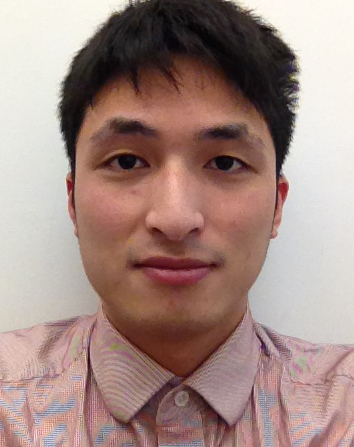
\includegraphics[width=1in,height=1.25in,clip,keepaspectratio]{author1}}]{Feng Liang}
is currently a PhD candidate in Department of Computer Science, The University of Hong Kong. He received his bachelor's degree in software engineering in Nanjing University in 2012. His research interests are mainly on distributed file systems, distributed computing, and machine learning. He is recently undertaking the research project on distributed deep learning.
[homepage] i.cs.hku.hk/\%7Efliang
\end{IEEEbiography}

\vspace{-0.5in}
\begin{IEEEbiography}[{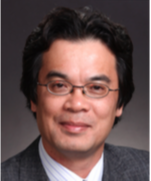
\includegraphics[width=1in,height=1.5in,clip,keepaspectratio]{author2}}]{Francis C.M. Lau}
received his PhD in computer science from the University of Waterloo in 1986. He has been a faculty member of the Department of Computer Science, The University of Hong Kong since 1987, where he served as the department chair from 2000 to 2005. He is now Associate Dean of Faculty of Engineering, the University of Hong Kong. He was a honorary chair professor in the Institute of Theoretical Computer Science of Tsinghua University from 2007 to 2010. His research interests include
computer systems and networking, algorithms, HCI, and application of IT to arts. He is the editor-in-chief of the Journal of Interconnection Networks.
[homepage] i.cs.hku.hk/\%7Efcmlau
\end{IEEEbiography}

\vspace{-0.5in}
\begin{IEEEbiography}[{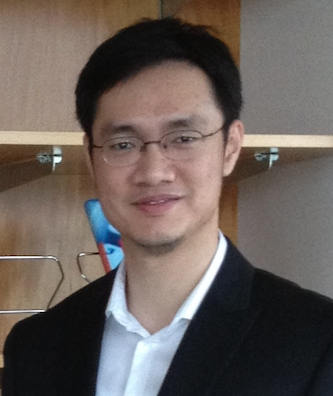
\includegraphics[width=1in,height=1.25in,clip,keepaspectratio]{author3}}]{Heming Cui}
is an assistant professor in Computer Science of HKU. His research interests are in operating systems, programming languages, distributed systems, and cloud computing, with a particular focus on building software infrastructures and tools to improve reliability and security of real-world software. 
[homepage] i.cs.hku.hk/\%7Eheming
\end{IEEEbiography}

\vspace{-0.5in}
\begin{IEEEbiography}[{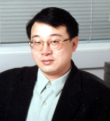
\includegraphics[width=1in,height=1.25in,clip,keepaspectratio]{author4}}]{Cho-Li Wang}
is currently a Professor in the Department of Computer Science at The
University of Hong Kong. He graduated with a B.S. degree in Computer Science and
Information Engineering from National Taiwan University in 1985 and a Ph.D.
degree in Computer Engineering from University of Southern California in 1995. Prof.
Wang’s research is broadly in the areas of parallel architecture, software systems for
Cluster computing, and virtualization techniques for Cloud computing. His recent
research projects involve the development of parallel software systems for
multicore/GPU computing and multi-kernel operating systems for future manycore
processor. Prof. Wang has published more than 150 papers in various peer reviewed
journals and conference proceedings. He is/was on the editorial boards of several scholarly
journals, including IEEE Transactions on Cloud Computing (2013-), IEEE
Transactions on Computers (2006-2010).
[homepage] i.cs.hku.hk/\%7Eclwang
\end{IEEEbiography}

% insert where needed to balance the two columns on the last page with
% biographies
%\newpage



% You can push biographies down or up by placing
% a \vfill before or after them. The appropriate
% use of \vfill depends on what kind of text is
% on the last page and whether or not the columns
% are being equalized.

%\vfill

% Can be used to pull up biographies so that the bottom of the last one
% is flush with the other column.
%\enlargethispage{-5in}



% that's all folks
\end{document}


